\documentclass[10pt,letterpaper]{article}
%\usepackage{toolsper}
%\settextfont{B Nazanin}
\usepackage{amsmath,amssymb,graphicx,geometry,tikz,diagbox,xepersian}
\usepackage{lipsum}
\setlength{\parindent}{0mm}
\setlength{\parskip}{3mm}

\newcounter{questionnumber}
\setcounter{questionnumber}{1}

\newcommand{\Q}{
\textbf{سوال \thequestionnumber)}
\stepcounter{questionnumber}
}

\newcommand{\pic}[2]{
\begin{center}
\includegraphics[width=#2]{#1}
\end{center}
}
\newcommand{\EX}{\mathbb{E}}
\newcommand{\eqn}[1]{
\[\begin{split}
#1
\end{split}\]
}


\begin{document}
\Large
\begin{center}

\hrulefill
\end{center}
سوال 1) دو کیسه در اختیار داریم. کیسه اول شامل 20 گلوله قرمز و 30 گلوله آبی و دومی شامل 20 گلوله زرد، 30 گلوله آبی و 50 گلوله قرمز است. ابتدا یکی از کیسه ها را به تصادف انتخاب کرده و سپس گلوله‌ای را از داخل آن به تصادف بر می داریم. با چه احتمالی گلوله انتخاب شده قرمز و از کیسه‌ی 2 است؟

سوال 2) تاس سالمی را 3 بار پرتاب می کنیم و اعداد رو آمده در سه پرتاب را در نظر می گیریم. احتمال آن که جمع اعداد رو آمده برابر 5 باشد چقدر است؟

سوال 3) برای تابع چگالی احتمال داده شده‌ی زیر:
$$
f_X(x)=\begin{cases}
k\delta(x+1)&,\quad x=-1\\
x-x^2&,\quad 0<x<1
\\0&,\quad \text{سایر جاها}
\end{cases}
$$

الف) مقدار k را بیابید.

ب) تابع توزیع تجمعی را بیابید.

پ) مقدار احتمال 
$
\Pr\{X^2\le 4\}
$
 را به دست آورید.

سوال 1) دو کیسه در اختیار داریم. کیسه اول شامل 20 گلوله قرمز و 30 گلوله آبی و دومی شامل 20 گلوله زرد، 30 گلوله آبی و 50 گلوله قرمز است. ابتدا یکی از کیسه ها را به تصادف انتخاب کرده و سپس گلوله‌ای را از داخل آن به تصادف بر می داریم. اگر گلوله از کیسه 1 انتخاب شده باشد، با چه احتمالی آبی است؟

سوال 2) تاس سالمی را 3 بار پرتاب می کنیم و اعداد رو آمده در سه پرتاب را در نظر می گیریم. اگر عدد رو آمده‌ی اول برابر 4 باشد، احتمال آن که جمع اعداد پرتاب ها برابر 7 باشد چقدر است؟

سوال 3) برای تابع چگالی احتمال داده شده‌ی زیر:

$$
f_X(x)=\begin{cases}
{1\over 2}\delta(x)&,\quad x=0\\
{3\over 32}\sqrt{x-1}&,\quad 1\le x\le k
\\0&,\quad \text{سایر جاها}
\end{cases}
$$

الف) مقدار k را بیابید.

ب) تابع توزیع تجمعی را بیابید.

پ) مقدار احتمال 
$
\Pr\{X^2\le 4\}
$
 را به دست آورید.

سوال 1) دو کیسه در اختیار داریم. کیسه اول شامل 20 گلوله قرمز و 30 گلوله آبی و دومی شامل 20 گلوله زرد، 30 گلوله آبی و 50 گلوله قرمز است. ابتدا یکی از کیسه ها را به تصادف انتخاب کرده و سپس گلوله‌ای را از داخل آن به تصادف بر می داریم. اگر گلوله زرد نباشد با چه احتمالی قرمز است؟

سوال 2) تاس سالمی را 3 بار پرتاب می کنیم و اعداد رو آمده در سه پرتاب را در نظر می گیریم. احتمال آن که جمع اعداد تاس در پرتاب های فرد، برابر 5 باشد چقدر است؟

سوال 3) برای تابع چگالی احتمال داده شده‌ی زیر:

$$
f_X(x)=\begin{cases}
k\delta(x+1)&,\quad x=-1\\
{1\over 2}{e^{-x+1}}&,\quad x\ge 1
\\0&,\quad \text{سایر جاها}
\end{cases}
$$

الف) مقدار k را بیابید.

ب) تابع توزیع تجمعی را بیابید.

پ) مقدار احتمال 
$
\Pr\{X^2\le 4\}
$
 را به دست آورید.

سوال 1) دو کیسه در اختیار داریم. کیسه اول شامل 20 گلوله قرمز و 30 گلوله آبی و دومی شامل 20 گلوله زرد، 30 گلوله آبی و 50 گلوله قرمز است. ابتدا یکی از کیسه ها را به تصادف انتخاب کرده و سپس گلوله‌ای را از داخل آن به تصادف بر می داریم. اگر گلوله آبی نباشد، با چه احتمالی از کیسه‌ی 2 انتخاب شده است؟

سوال 2) تاس سالمی را 4 بار پرتاب می کنیم و اعداد رو آمده در چهار پرتاب را در نظر می گیریم. اگر در دو پرتاب این تاس عدد 2 ظاهر شده باشد، احتمال آنکه در دو پرتاب دیگر عدد فردی ظاهر شده باشد چقدر است؟

سوال 3) برای تابع چگالی احتمال داده شده‌ی زیر:

$$
f_X(x)=\begin{cases}
{1\over 2}\delta(x+3)&,\quad x=-3\\
{1\over 2}\sin x&,\quad 0\le x\le k
\\0&,\quad \text{سایر جاها}
\end{cases}
$$

الف) مقدار k را بیابید.

ب) تابع توزیع تجمعی را بیابید.

پ) مقدار احتمال 
$
\Pr\{X^2\le 4\}
$
 را به دست آورید.

سوال 1)

%کشوری شامل دو استان است. استان 1 شامل 100 مرد و 100 زن و استان 2 شامل 200 مرد و 150 زن می باشد. 30 مرد و 20 زن از استان 1 و  فردی را به تصادف از این کشور بر می گزینیم.

دو کیسه در اختیار داریم. کیسه اول شامل 20 گلوله قرمز و 30 گلوله آبی و دومی شامل 20 گلوله زرد، 30 گلوله آبی و 50 گلوله قرمز است. ابتدا یکی از کیسه ها را به تصادف انتخاب کرده و سپس گلوله‌ای را از داخل آن به تصادف بر می داریم. اگر گلوله قرمز یا زرد نباشد، با چه احتمالی از کیسه 2 انتخاب شده است؟

سوال 2) تاس سالمی را 4 بار پرتاب می کنیم و اعداد رو آمده در چهار پرتاب را در نظر می گیریم. با چه احتمالی، جمع اعداد در پرتاب های زوج، 5 برابر جمع اعداد در پرتاب های فرد  است؟

سوال 3) برای تابع چگالی احتمال داده شده‌ی زیر:

$$
f_X(x)=\begin{cases}
{1\over 2}\delta(x+1)&,\quad x=-1\\
{1\over x^3}&,\quad x\ge k
\\0&,\quad \text{سایر جاها}
\end{cases}
$$
الف) مقدار k را بیابید.

ب) تابع توزیع تجمعی را بیابید.

پ) مقدار احتمال 
$
\Pr\{X^2\le 4\}
$
 را به دست آورید.

سوال 1) تابع چگالی احتمال توام دو متغیر تصادفی $X$ و $Y$ به صورت زیر است:
$$
f(x,y)=
\begin{cases}
k(4-x-y) &,\quad 1 < x < 2\ \ ,\ \   0 < y < 2 \\
0 &,\quad \text{\rl{در غیر این صورت}}
\end{cases}
$$
الف) مقدار مناسب $k$ را بیابید.

ب) با مقدار $k$ به دست آمده در قسمت قبل، مقدار 
$
\EX \{XY\}
$
 را به دست آورید.

سوال 2) فرض کنید دنباله‌ی متغیرهای تصادفی 
$
\{
X_n
\}
$
، از توزیع یکنواخت بین 
$
-{1\over 2}
$
 و $1\over 2$ و به طور مستقل پیروی می‌کند. به کمک قضیه‌ی حد مرکزی، توزیع متغیر تصادفی $Y$ را به دست آورید که 
$$
Y=\lim_{n\to \infty} {X_1+X_2+\cdots +X_n\over \sqrt n}
$$
و میانگین و واریانس آن را بیابید.

سوال 3) فرض کنید متغیر تصادفی $X$، یکنواخت در بازه‌ی $[0,1]$ است. متغیر تصادفی $Y$ را به صورت $Y=g(X)$ می سازیم. تابع $g$ را به گونه ای تعیین کنید که $Y$:

الف) یک متغیر تصادفی نمایی با پارامتر 1 باشد؛ یعنی
$$
f(y)=\begin{cases}
e^{-y}&,\quad y>0\\
0&,\quad y\le 0
\end{cases}
$$
ب) یک متغیر تصادفی کوشی با پارامتر $\pi$ باشد؛ یعنی
$$
f(y)={1\over y^2+\pi^2}\quad,\quad y\in\Bbb R
$$

سوال 4) تابع چگالی احتمال توام دو متغیر تصادفی $X$ و $Y$ به صورت زیر است:
$$
f(x,y)=
\begin{cases}
1 &,\quad |x|+2|y|<1\\
0 &,\quad |x|+2|y|\ge 1
\end{cases}
$$
الف)  چگالی های احتمال حاشیه ای $X$ و $Y$ را به دست آورید. همچنین ناهمبستگی، استقلال و تعامد این دو متغیر تصادفی را تحقیق کنید.

ب) چگالی احتمال $X+Y$ را به دست آورید.

سوال 5) یک قطار و اتوبوس به طور تصادفی و مستقل از هم بین ساعات 5 تا 6 وارد یک ایستگاه می شوند. فردی نیز به طور تصادفی بین ساعت 5 تا $5:30$ وارد همان ایستگاه می شود.

الف) احتمال آن که فرد بیش از 10 دقیقه منتظر قطار و اتوبوس شود چقدر است؟

ب) اگر قطار و اتوبوس هر یک 10 دقیقه در ایستگاه تاخیر داشته باشند، احتمال با هم بودن آنها در ایستگاه چفدر است؟

پ) اگر فرد پس از ساعت $5:15$ به ایستگاه برسد، با چه احتمالی به هیچ یک نمی رسد؟

سوال 6) متغیر تصادفی و گسسته‌ی $N$ دارای چگالی احتمال زیر است:
$$
f(n)=\begin{cases}
n\left({1\over 2}\right)^{n+1}&,\quad n\in \Bbb N\\
0&,\quad \text{\rl{در غیر این صورت}}
\end{cases}
$$
الف) تابع مولد گشتاور آن را به دست آورید.

ب) از روی تابع مولد گشتاور، مقادیر میانگین و واریانس این متغیر تصادفی را محاسبه کنید.

(راهنمایی: 
$$
\sum_{n=1}^{\infty} na^n={a\over (1-a)^2}\quad,\quad |a|<1
$$
)

سوال 7) اگر $X$ و $Y$، دو متغیر تصادفی نرمال با میانگین 0 و واریانس 1 باشند به گونه ای که 
$
\text{\lr{cov}}(X,Y)=0.5
$
، در این صورت مقدار $a$  را به گونه ای بیابید که $X+aY$ و $X+2Y$ مستقل از هم باشند و در این صورت، واریانس هر یک را بیابید.

سوال 8) تاس سالمی را 9 بار پرتاب می‌کنیم. اگر متغیر تصادفی $X$، تعداد اعداد زوج رو آمده به شرط دانستن این باشد که در سه پرتاب اول، حداقل یک عدد فرد آمده است،

الف)  چگالی احتمال $X$ را محاسبه کنید.

ب) اگر متغیر تصادفی $Y$، تعداد اعداد اول رو آمده باشد، مقدار 
$
\Pr\{X=x|Y=0\}
$
 چقدر است؟

سوال 9)

الف) تابع مولد گشتاور متغیر تصادفی پواسون با پارامتر $\lambda$  را به دست آورید.

ب) اگر دنباله‌ی متغیرهای تصادفی مستقل $\{X_n\}$، از نوع پواسون با پارامتر $\lambda$ باشد، نشان دهید متغیر تصادفی 
$$
Y=\sum_{i=1}^NX_i
$$
، پواسون با پارامتر $N\lambda$ است.

پ) نشان دهید اگر دنباله‌ی متغیرهای تصادفی مستقل $\{X_n\}$، برنولی با پارامتر $p$ و $N$ از نوع پواسون با پارامتر $\lambda$ باشد، متغیر تصادفی
$$
Y=\sum_{n=0}^{N-1} X_n
$$
 دارای توزیع پواسون با پارامتر $\lambda p$ است.

سوال 10) نشان دهید دنباله‌ی متغیرهای تصادفی 
$
X_n=X+{1\over n}
$
که $n$ عدد طبیعی و $X$ دارای توزیع یکنواخت بین 0 و 1 است، در احتمال به $X$ میل می کند.

سوال 11) فرض کنید برای یک متغیر تصادفی با چگالی توزیع $f(x)$ داشته باشیم
$$
\exists a\in\Bbb R \quad,\quad  f(x)=f(a-x)
$$
نشان دهید میانگین و میانه‌ی این متغیر تصادفی برابر $a$ است.

سوال 1) تابع چگالی احتمال توام دو متغیر تصادفی $X$ و $Y$ به صورت زیر است:
$$
f(x,y)=
\begin{cases}
k(4-x-y) &,\quad 1 < x < 2\ \ ,\ \   0 < y < 2 \\
0 &,\quad \text{\rl{در غیر این صورت}}
\end{cases}
$$
الف) مقدار مناسب $k$ را بیابید.

ب) با مقدار $k$ به دست آمده در قسمت قبل، مقدار 
$
\EX \{XY\}
$
 را به دست آورید.

سوال 2) فرض کنید دنباله‌ی متغیرهای تصادفی 
$
\{
X_n
\}
$
، از توزیع یکنواخت بین 
$
-{1\over 2}
$
 و $1\over 2$ و به طور مستقل پیروی می‌کند. به کمک قضیه‌ی حد مرکزی، توزیع متغیر تصادفی $Y$ را به دست آورید که 
$$
Y=\lim_{n\to \infty} {X_1+X_2+\cdots +X_n\over \sqrt n}
$$
و میانگین و واریانس آن را بیابید.

سوال 3) فرض کنید متغیر تصادفی $X$، یکنواخت در بازه‌ی $[0,1]$ است. متغیر تصادفی $Y$ را به صورت $Y=g(X)$ می سازیم. تابع $g$ را به گونه ای تعیین کنید که $Y$:

الف) یک متغیر تصادفی نمایی با پارامتر 1 باشد؛ یعنی
$$
f(y)=\begin{cases}
e^{-y}&,\quad y>0\\
0&,\quad y\le 0
\end{cases}
$$
ب) یک متغیر تصادفی کوشی با پارامتر $\pi$ باشد؛ یعنی
$$
f(y)={1\over y^2+\pi^2}\quad,\quad y\in\Bbb R
$$

سوال 4) تابع چگالی احتمال توام دو متغیر تصادفی $X$ و $Y$ به صورت زیر است:
$$
f(x,y)=
\begin{cases}
1 &,\quad |x|+2|y|<1\\
0 &,\quad |x|+2|y|\ge 1
\end{cases}
$$
الف)  چگالی های احتمال حاشیه ای $X$ و $Y$ را به دست آورید. همچنین ناهمبستگی، استقلال و تعامد این دو متغیر تصادفی را تحقیق کنید.

ب) چگالی احتمال $X+Y$ را به دست آورید.

سوال 5) یک قطار و اتوبوس به طور تصادفی و مستقل از هم بین ساعات 5 تا 6 وارد یک ایستگاه می شوند. فردی نیز به طور تصادفی بین ساعت 5 تا $5:30$ وارد همان ایستگاه می شود.

الف) احتمال آن که فرد بیش از 10 دقیقه منتظر قطار و اتوبوس شود چقدر است؟

ب) اگر قطار و اتوبوس هر یک 10 دقیقه در ایستگاه تاخیر داشته باشند، احتمال با هم بودن آنها در ایستگاه چفدر است؟

پ) اگر فرد پس از ساعت $5:15$ به ایستگاه برسد، با چه احتمالی به هیچ یک نمی رسد؟

سوال 6) متغیر تصادفی و گسسته‌ی $N$ دارای چگالی احتمال زیر است:
$$
f(n)=\begin{cases}
n\left({1\over 2}\right)^{n+1}&,\quad n\in \Bbb N\\
0&,\quad \text{\rl{در غیر این صورت}}
\end{cases}
$$
الف) تابع مولد گشتاور آن را به دست آورید.

ب) از روی تابع مولد گشتاور، مقادیر میانگین و واریانس این متغیر تصادفی را محاسبه کنید.

(راهنمایی: 
$$
\sum_{n=1}^{\infty} na^n={a\over (1-a)^2}\quad,\quad |a|<1
$$
)

سوال 7) اگر $X$ و $Y$، دو متغیر تصادفی نرمال با میانگین 0 و واریانس 1 باشند به گونه ای که 
$
\text{\lr{cov}}(X,Y)=0.5
$
، در این صورت مقدار $a$  را به گونه ای بیابید که $X+aY$ و $X+2Y$ مستقل از هم باشند و در این صورت، واریانس هر یک را بیابید.

سوال 8) تاس سالمی را 9 بار پرتاب می‌کنیم. اگر متغیر تصادفی $X$، تعداد اعداد زوج رو آمده به شرط دانستن این باشد که در سه پرتاب اول، حداقل یک عدد فرد آمده است،

الف)  چگالی احتمال $X$ را محاسبه کنید.

ب) اگر متغیر تصادفی $Y$، تعداد اعداد اول رو آمده باشد، مقدار 
$
\Pr\{X=x|Y=0\}
$
 چقدر است؟

سوال 9)

الف) تابع مولد گشتاور متغیر تصادفی پواسون با پارامتر $\lambda$  را به دست آورید.

ب) اگر دنباله‌ی متغیرهای تصادفی مستقل $\{X_n\}$، از نوع پواسون با پارامتر $\lambda$ باشد، نشان دهید متغیر تصادفی 
$$
Y=\sum_{i=1}^NX_i
$$
، پواسون با پارامتر $N\lambda$ است.

پ) نشان دهید اگر دنباله‌ی متغیرهای تصادفی مستقل $\{X_n\}$، برنولی با پارامتر $p$ و $N$ از نوع پواسون با پارامتر $\lambda$ باشد، متغیر تصادفی
$$
Y=\sum_{n=0}^{N-1} X_n
$$
 دارای توزیع پواسون با پارامتر $\lambda p$ است.

سوال 10) نشان دهید دنباله‌ی متغیرهای تصادفی 
$
X_n=X+{1\over n}
$
که $n$ عدد طبیعی و $X$ دارای توزیع یکنواخت بین 0 و 1 است، در احتمال به $X$ میل می کند.

سوال 11) فرض کنید برای یک متغیر تصادفی با چگالی توزیع $f(x)$ داشته باشیم
$$
\exists a\in\Bbb R \quad,\quad  f(x)=f(a-x)
$$
نشان دهید میانگین و میانه‌ی این متغیر تصادفی برابر $a$ است.

سوال 1) استانی دارای دو شهر است. شهر 1 دارای 120 مرد و 80 زن و شهر 2 دارای 1000 زن و 800 مرد است. در شهر 1،  50 مرد و 30 زن و در شهر 2، 100 مرد و 150 زن به بیماری X مبتلا هستد. فردی را از این استان به تصادف انتخاب می کنیم.

الف) با چه احتمالی این فرد، زن سالمی از شهر 1 است؟

ب) اگر فردی که انتخاب می کنیم بیمار باشد، با چه احتمالی مردی از شهر 2 است؟

%پ) اگر فرد انتخاب شده سالم باشد، احتمال زن بودن او چقدر است؟
\newpage
سوال 2) یک قطار و اتوبوس به طور تصادفی و مستقل از هم بین ساعات 6 تا 7 صبح وارد ایستگاهی می شوند. فردي نیز به طور تصادفی بین ساعات 5:50 تا 6:50 وارد همان ایستگاه می شود.

الف) احتمال اینکه فرد بیش از 10 دقیقه منتظر قطار ویا اتوبوس بماند چقدر است؟

ب) احتمال اینکه این فرد به هیچ یک از قطار یا اتوبوس نرسد چقدر است؟
\newpage
سوال 3) متغیر تصادفی $X$ با تابع توزیع تجمعی زیر داده شده است:
$$
F_X(x)=\begin{cases}
1-{x+1\over 2}e^{-x}&,\quad x\ge 0
\\0&,\quad x<0
\end{cases}
$$
در این صورت

الف) تابع مولد گشتاور آن را به دست آورید.

ب) میانگین و واریانس این متغیر تصادفی را بیابید.
\newpage
سوال 4) سکه ای را 10 بار پرتاب می کنیم. متغیر تصادفی $X$ برابر تعداد دفعات رو آمدن در پرتاب های دوم و چهارم و متغیر تصادفی $Y$ برابر تعداد دفعات پشت آمدن در 2 پرتاب اول است.

الف) چگالی احتمال شرطی
$
f_{X|Y}(X=x|Y=y)
$
 را به دست آورید (می توانید از روش جدول نویسی برای چگالی احتمال استفاده کنید که سطر جدول $X=x$ و ستون جدول $Y=y$ است).

ب) مقدار 
$
E\{XY\}
$
 را بیابید.
\newpage
سوال 5) تابع چگالی احتمال توأم دو متغیر تصادفی $X$ و $Y$ به صورت زیر است:
$$
f_{X,Y}(x,y)=\begin{cases}
k&,\quad x-1<y<x\ \ ,\ \ 0<x<2\ \ ,\ \ 0<y<1
\\0&,\quad \text{در غیر این صورت}
\end{cases}
$$
که $k$ ثابت است.

الف) مقدار $k$ را به دست آورید.

ب) نشان دهید $Y$ و $X-Y$ از هم مستقل هستند.

سوال 1) یک سکه سالم را برداشته، آن را سه بار پرتاب می کنیم و نتیجه‌ی سه بار پرتاب را در نظر می‌گیریم. اگر رو آمدن سکه را با H و پشت آمدن را با T نمایش دهیم:

الف) فضای نمونه را بیابید.

ب) این مسئله ی احتمال، چند واقعه‌ی محتمل دارد؟ (واقعه طبق تعریف یک زیر مجموعه از فضای نمونه است).

پ) طبق تعریف کلاسیک احتمال، واقعه‌ی اینکه در پرتاب اول و دوم سکه نتیجه یکسان باشد (در پرتاب سوم نتیجه دلخواه است)، با چه احتمالی رخ می دهد؟

سوال 2) دو مجموعه‌ی 
$
A=\{1,4,5\}
$
و
$
B=\{2,3,4\}
$
 را در نظر بگیرید. مجموعه های زیر را به دست آورید.

الف) 
$
A\cap B
$

ب)
$
A-B
$

پ)
$
A\times B
$
 (ضرب دکارتی)

ت) اگر 
$
C=\{2,5,6\}
$
، با محاسبه‌ی مجموعه های 
$
(A\cup B)\cap C
$
و
$
(A\cap C)\cup (B\cap C)
$
نشان دهید:
$$
(A\cup B)\cap C=(A\cap C)\cup (B\cap C)
$$

سوال 3) به کمک تعریف اصولی احتمال (و با بهره گیری از اصول کولموگروف)، برای هر دو مجموعه‌ی A و B نتیجه بگیرید:
$$
P(A)=P(A-B)+P(A\cap B)
$$
%%به دست آورید (جایگذاری حالتی است که گلوله ای را پس از بیرون آوردن از کیسه و مشاهده‌ی رنگ آن، به کیسه باز گردانیم).
%
%سوال 2) در نقشه‌ی زیر، از شهر $A$ به شهر $B$ دو مسیر و از $B$ به $C$ یا از $A$ به $C$ یک مسیر وجود دارد. اگر احتمال قطع شدن هر مسیر مستقل از سایرین برابر $p$ باشد، احتمال آن که شخصی بتواند از شهر $A$ به $C$ برود چقدر است؟
%\pic{Q2.pdf}{100mm}
%
%سوال 3) در مبحث مدولاسیون دیجیتال، می‌توان هر سمبل مخابراتی را با تعدادی بیت کد نموده و پس از شکل دهی پالس روی کانال ارسال کرد. فرض کنید یک سمبل مخابراتی از $n$ بیت تشکیل شده باشد. به طور مثال
%\eqn{
%S_k\equiv (1010001101)_2
%}{}
%که $k$ اندیس سمبل است و در اینجا سمبل از $10$ بیت تشکیل شده است. این سمبل از یک کانال مخابراتی ارسال و در انتهای کانال دریافت می‌شود. اگر احتمال خرابی هر بیت مستقل از سایرین برابر $p$ باشد، با چه احتمالی سمبل به درستی آشکار \underline{نمی‌شود}؟
%
%سوال 4) دو تاس را پرتاب می‌کنیم. احتمال اینکه دو عدد رو آمده نسبت به هم اول باشند چقدر است؟
%
%سوال 5) از یک مجموعه‌ی $n$ عضوی، یک زیر مجموعه‌ به تصادف انتخاب می‌کنیم. احتمال آن که این زیر مجموعه $k$ عضوی باشد چقدر است؟
%
%سوال 6) به کمک سوال قبل ثابت کنید
%\eqn{
%\sum_{k=0}^n\binom{n}{k}=2^n
%}{}

سوال 1) در یک کیسه، 5 گلوله‌ی آبی و 3 گلوله‌ی سفید وجود دارد. دو عدد گلوله بر می‌داریم. احتمال این را که یکی از گلوله ها آبی و دیگری سفید باشد در حالت
\newline
الف) با جایگذاری
\newline
ب) بدون جایگذاری
\newline
به دست آورید (جایگذاری حالتی است که گلوله ای را پس از بیرون آوردن از کیسه و مشاهده‌ی رنگ آن، به کیسه باز گردانیم).

سوال 2) در نقشه‌ی زیر، از شهر $A$ به شهر $B$ دو مسیر و از $B$ به $C$ یا از $A$ به $C$ یک مسیر وجود دارد. اگر احتمال قطع شدن هر مسیر مستقل از سایرین برابر $p$ باشد، احتمال آن که شخصی بتواند از شهر $A$ به $C$ برود چقدر است؟
\pic{Q2.pdf}{100mm}

سوال 3) در مبحث مدولاسیون دیجیتال، می‌توان هر سمبل مخابراتی را با تعدادی بیت کد نموده و پس از شکل دهی پالس روی کانال ارسال کرد. فرض کنید یک سمبل مخابراتی از $n$ بیت تشکیل شده باشد. به طور مثال
\eqn{
S_k\equiv (1010001101)_2
}{}
که $k$ اندیس سمبل است و در اینجا سمبل از $10$ بیت تشکیل شده است. این سمبل از یک کانال مخابراتی ارسال و در انتهای کانال دریافت می‌شود. اگر احتمال خرابی هر بیت مستقل از سایرین برابر $p$ باشد، با چه احتمالی سمبل به درستی آشکار \underline{نمی‌شود}؟

سوال 4) دو تاس را پرتاب می‌کنیم. احتمال اینکه دو عدد رو آمده نسبت به هم اول باشند چقدر است؟

سوال 5) از یک مجموعه‌ی $n$ عضوی، یک زیر مجموعه‌ به تصادف انتخاب می‌کنیم. احتمال آن که این زیر مجموعه $k$ عضوی باشد چقدر است؟

سوال 6) به کمک سوال قبل ثابت کنید
\eqn{
\sum_{k=0}^n\binom{n}{k}=2^n
}{}

سوال 1) یک سکه‌ی سالم و یک تاس سالم را با هم پرتاب می کنیم.

الف) احتمال اینکه سکه به رو بیفتد و تاس عدد فرد شود را به دست آورید.

ب) احتمال اینکه سکه به رو بیفتد یا تاس عدد فرد شود را به دست آورید (هر دو باهم نیز می توانند رخ دهند!)

سوال 2) یک تاس را پرتاب می کنیم. اگر مضرب 3 ظاهر شد، نتیجه را یادداشت می کنیم و در غیر این صورت سکه ای را می اندازیم و نتیجه‌ی سکه (پشت یا رو) را می نویسیم.

الف) فضای شدنی این مسئله را بیابید.

ب) با چه احتمالی واقعه‌ی رو آمدن سکه اتفاق می افتد؟

پ) احتمال واقعه‌ی اینکه تاس عدد 1 بیاید یا سکه به پشت ظاهر شود را به دست آورید.

سوال 3) نقطه ای را از داخل مربع زیر بر می گزینیم (طول ضلع مربع برابر 2 است). احتمال اینکه:

\begin{figure}[h!]
\centering
\includegraphics[width=130mm]{figure_1}
\end{figure}

الف) نقطه، داخل دایره ی واحد (نشان داده شده در شکل) بیفتد چقدر است؟

ب) نقطه، روی یکی از دو قطر مربع بیفتد چقدر است؟

پ) فاصله‌ی نقطه از هر یک از رأس های مربع بیش از 0/5 باشد چقدر است؟

سوال 4) از بین اعداد سه رقمی ای که با ترکیب رقم های 0، 1 و  2 می توان ساخت (تکرار مجاز است):

الف) چند عدد به 3 بخش پذیرند؟

ب) اگر عددی را به تصادف برگزینیم، با چه احتمالی زوج خواهد بود؟

سوال 1) در یک جامعه‌ی آماری، نسبت جمعیت زنان بزرگسال، مردان بزرگسال و کودکان به کل جمعیت جامعه به ترتیب برابر $0.37$، $0.43$ و $0.2$ است. در این جامعه، $0.15$ مردان بزرگسال و $0.25$ زنان بزرگسال به نوعی بیماری مبتلا شده اند. فرد بزرگسالی را به تصادف از این جامعه انتخاب می‌کنیم، احتمال بیمار بودن او چقدر است؟

سوال 2) فرض کنید مجموعه های B و C مستقل و دارای احتمال مثبت باشند. در چه حالتی داریم
$$
P(A|B\cap C)=P(A|B)P(A|C)
$$
؟

سوال 3) (کران بالا و پایین برای احتمال اجتماع) برای هر دو مجموعه‌ی A و B ثابت کنید:
$$
P(A)+P(B)-\frac{1}{4\max\{1-P(A),1-P(B)\}}
\le 
P(A\cup B)
\le 
P(A)+P(B)
$$

سوال 13) نشان دهید که اگر به ازای هر $t_0$ و $t_1$ مثبتی داشته باشیم
$$
\Pr\{t_0\le t\le t_0+t_1|t\ge t_0\}=\Pr\{t\le t_1\}
$$
آنگاه 
$$
\Pr\{t\le t_1\}=1-e^{-ct_1}
$$

سوال 22) نشان دهید که برای استقلال $n$ رخداد باید 
$2^n-n-1$
 معادله برقرار باشد.

سوال 24) جعبه‌ی 1 حاوی 1000 لامپ است که 10 درصد آنها خراب هستند. جعبه‌ی 2 نیز حاوی 2000 لامپ است که 5 درصد آنها خراب هستند. از یک جعبه که به طور تصادفی انتخاب شده، دو لامپ بیرون آورده می شوند.

الف) احتمال خرابی هر دو چقدر است؟

ب) اگر هر دو لامپ خراب باشند، با چه احتمالی جعبه‌ی 1 انتخاب شده است؟

سوال 25) یک قطار و یک اتوبوس بین ساعت $9$ و $10$ در زمانی تصادفی وارد ایستگاه می شوند. قطار $10$ دقیقه و اتوبوس $x$ دقیقه توقف دارند. $x$ را طوری تعیین کنید که احتمال با هم بودن قطار و اتوبوس برابر $0.5$ باشد.

سوال 1) در یک کیسه، 5 گلوله ي آبی و 3 گلوله ي سفید وجود دارد. دو عدد گلوله بر می داریم. احتمال
این را که یکی از گلوله ها آبی و دیگري سفید باشد در حالت

الف) با جایگذاري

ب) بدون جایگذاري

به دست آورید (جایگذاري حالتی است که گلوله اي را پس از بیرون آوردن از کیسه و مشاهده ي رنگ آن،
به کیسه باز گردانیم).

سوال 2) سکه‌ی سالمی را 10 بار پرتاب می کنیم. مطلوبست احتمال آن که

الف) در این 10 پرتاب، حداقل دوبار رو بیاید.

ب) در سه پرتاب اول حداکثر یک بار پشت بیاید.

پ) در پرتاب های زوج، نتیجه یکسان باشد (همگی رو یا همگی پشت باشند).

سوال 3) در یک گل فروشی، 10 گل لاله، 5 نسترن، 3 بنفشه و 2 اقاقیا وجود دارد. می خواهیم دسته گلی شامل 5 گل که همگی به تصادف انتخاب شده باشند، برگزینیم. با چه احتمالی

الف) دسته گل شامل 2 نسترن و 2 بنفشه است؟

ب) دسته گل شامل هیچ گل لاله و بنفشه ای نیست؟

پ) دسته گل شامل حداقل یک گل از هر یک از 4 نوع گل است؟

(دقت کنید گل های هر نوع با هم فرقی نمی کنند!)

سوال 4)

الف) از یک مجموعه‌ی $n$ عضوي، یک زیر مجموعه به تصادف انتخاب می کنیم. احتمال آن که این زیر مجموعه $k$ عضوي باشد چقدر است؟

ب) به کمک قسمت قبل ثابت کنید:
$$
\sum_{k=0}^n\binom{n}{k}=2^n
$$

سوال 5)

الف) اگر یک رشته لامپ متوالی شامل $n$ لامپ که هر لامپ به احتمال $p$ خراب است، به ولتاژ برق وصل شود، با چه احتمالی روشن می شود؟ (در رشته متوالی لامپ ها، لامپ ها به صورت پشت سر هم به یکدیگر وصل شده اند)

ب) اگر رشته لامپ موازی باشد، مسئله را حل کنید. (در رشته‌ی موازی لامپ ها، یکی از سرهای همه‌ی لامپ ها به یک نقطه و سر دیگر تمام لامپ ها به نقطه‌ی دیگر وصل شده اند)

سوال 1) (امتیازی)

الف) قضیه‌ی دموآو-لاپلاس در چه حالتی برای تکرر توزیع برنولی به تعداد $n$ بار برقرار است؟

ب) توزیع دوجمله ای را با پارامترهای $n=1000$ و $p=0.5$ در نظر بگیرید. به کمک ماشین حساب یا کامپیوتر، خطای نسبی تقریب قضیه‌ی دموآو-لاپلاس را برای $k=1,300,490$ محاسبه کنید.

سوال 2) 

از یک جعبه که دارای $M$ گلوله‌ی سفید و $N-M$ گلوله‌ی سیاه است، $n$ گلوله برداشته می شود.

الف)
احتمال آنکه $m$ گلوله از گلوله های برداشته شده سفید باشند در حالت با جایگذاری چقدر است؟

ب)
احتمال آنکه $m$ گلوله از گلوله های برداشته شده سفید باشند در حالت بدون جایگذاری چقدر است؟

ج) اگر بدانیم تمام گلوله های سفید برداشته شده اند، احتمال آنکه دقیقا 2 گلوله‌ی سیاه نیز برداشته شده باشند چقدر است؟

سوال 3) (قدم زدن تصادفی) 

فردی از نقطه‌ی صفر روی محور اعداد حقیقی با احتمال $p$ یک متر به سمت راست و با احتمال $1-p$ یک متر به سمت چپ می  رود. اگر این فرد این نوع قدم زدن را $n$ بار و هربار از روی نقطه ای که روی آن ایستاده تکرار کند، با چه احتمالی پس از $k$ بار قدم زدن به مبدا باز می گردد؟

سوال 4) 

از مجموعه‌ی
 $
S=\{1,2,3,\cdots ,n\}
$
 دو زیر مجموعه به تصادف و به طور مستقل بر می‌گزینیم به گونه ای که احتمال آن که هر عضو $S$ داخل هر یکی از زیر مجموعه ها باشد، مستقل از دیگر اعضا برابر $p$ است. با چه احتمالی این دو زیرمجموعه ناسازگار هستند؟

سوال 5) 

دو تیم ورزشی $A$ و $B$ در یک بازی در 9 دست با هم روبرو می شوند و نتیجه‌ی هر دست فقط برد یکی از دو تیم می تواند باشد. فرض کنید تیم $A$ با احتمال $p$ در هر دست پیروز می شود و نتیجه‌ی دست ها مستقل از هم است. برنده‌ی بازی کسی است که بیشتر بازی ها را برده باشد.

الف) با چه احتمالی تیم $A$ پس از 6 بازی موفق به بردن بازی می شود؟

ب) اگر بدانیم تیم $A$ در نهایت بازی را برده است، با چه احتمالی در حداقل یک دست به تیم $B$ باخته است؟

ج) به ازای $p=0.5$، اگر بدانیم تیم $A$ دست اول را برده، با چه احتمالی بازی را می برد؟

سوال 6)

در یک امتحان، احتمال درست پاسخ دادن به یک سوال دو گزینه ای برابر $p$ است. پس از امتحان، $n$ دانشجو پاسخ های خود را با هم مقایسه می کنند و متوجه می شوند که همگی به آن سوال پاسخ یکسانی داده اند. با چه احتمالی تمام این $n$ دانشجوها به پاسخ درست رسیده اند؟

سوال 1) احتمال اینکه فردی به
\lr{covid-19}
 مبتلا شود، در صورتی که ماسک نزند برابر $70\%$ و در صورتی که ماسک بزند برابر $15\%$ است. اگر این فرد به طور متوسط $5\%$ مواقع ماسک بزند، احتمال کرونا گرفتن او چقدر است؟

سوال 2) دو تاس می اندازیم و جمع دو عدد رو آمده را یادداشت می کنیم.

الف) احتمال اینکه عدد رو آمده، زوج باشد چقدر است؟

ب) اگر جمع دو عدد رو آمده زوج باشد، با چه احتمالی بیشتر از 8 است؟

سوال 3) از بین $2^n$ زیرمجموعه‌ی مجموعه‌ی $S=\{1,2,\cdots,n\}$، دو زیر مجموعه به تصادف و مستقل از هم بر می داریم. اگر این دو زیر مجموعه، دارای اشتراک $\{1,2\}$ باشند، احتمال آن که یکی از زیرمجموعه‌ها شامل عضوهای 3، 4 و 5 باشد چقدر است؟ ($n\ge 5$)

سوال 4) سه جعبه در اختیار داریم. در جعبه‌ی 1، 1000 لامپ موجود است که 3تای آنها معیوبند. جعبه‌ی 2 شامل 10 لامپ است که 3 تای آنها معیوبند و در جعبه‌ی سوم هم 3000 لامپ وجود دارد که همگی سالمند. اگر یکی از این جعبه ها را به تصادف برگزیده و از داخل آن لامپی انتخاب کنیم،

الف) با چه احتمالی لامپ معیوب است؟

ب) اگر لامپ معیوب باشد، با چه احتمالی از جعبه‌ی 2 انتخاب شده است؟

پ) اگر لامپ سالم باشد، با چه احتمالی از یکی از جعبه‌های 1 یا 2 انتخاب شده است؟

سوال 5) کشوری شامل دو استان 1 و 2 است. استان 1، شامل 60 مرد و 40 زن و استان 2 شامل 650 زن و 350 مرد است. در استان 1، 10 مرد و 10 زن چشم آبی و در استان 2، 30 مرد و 20 زن چشم آبی هستند. فردی را به تصادف از این کشور انتخاب می کنیم.

الف) اگر این فرد چشم آبی باشد، با چه احتمالی از استان 1 انتخاب شده است؟

ب) اگر این فرد زن باشد، با چه احتمالی از استان 2 انتخاب شده و چشم آبی \underline{نیست}؟

پ) اگر فرد انتخاب شده مرد باشد، با چه احتمالی چشم آبی است؟

سوال 1) فرض کنید تابع توزیع تجمعی یک متغیر تصادفی گسسته به صورت های زیر داده شده باشد:

الف) 
$
F(n)=\Pr\{X\le n\}=\begin{cases}
1&,\quad n> b
\\
{n-a+1\over b-a+1}&,\quad a\le n\le b
\\
0&,\quad n<a
\end{cases}
$
 زمانی که $b\ge a$

ب) 
$
F(n)=
\begin{cases}
1-A^{n+1}&,\quad n\ge 0
\\
0&,\quad \text{\rl{در غیر این صورت}}
\end{cases}
$
 زمانی که $0<A<1$

کمیت
$
f(n)=F(n)-F(n-1)
$
 را  محاسبه کرده و سپس $
\sum_{n=-\infty}^{\infty} nf(n)
$
 را برای این دو توزیع به دست آورید.

سوال 2) تابع توزیع های تجمعی و پیوسته ی زیر را در نظر بگیرید:

 الف) 
$
F(x)=\begin{cases}1-e^{-{1\over \lambda}x}&,\quad x>0
\\0&,\quad \text{\rl{در غیر این صورت}}
\end{cases}
$ 
زمانی که $\lambda>0$

ب) 
$
F(x)=\begin{cases}
1&,\quad x\ge b
\\{x-a\over b-a}&,\quad a<x<b
\\0&,\quad x\le a
\end{cases}
$
 زمانی که $b>a$

ج) 
$
F(x)={1\over \sqrt{2\pi\sigma^2}}\int_{-\infty}^x e^{-{(t-\mu)^2\over 2\sigma^2}}dt
$
 که $\mu$ و $\sigma^2$ دو مقدار حقیقی هستند و $\sigma^2\ne 0$

کمیت 
$
f(x)={dF(x)\over dx}
$
 را محاسبه کرده و از روی آن، 
$
\int_{-\infty}^\infty xf(x)dx
$
 را برای این سه توزیع به دست آورید.

سوال 3) فرض کنید $X$ و $Y$ دو متغیر تصادفی مستقل برنولی به ترتیب با پارامترهای $1\over 2$ و $p$ باشند. ثابت کنید متغیر تصادفی 
$
Z=X\oplus Y \mod 2
$
 دارای توزیع برنولی با پارامتر $1\over 2$ است.

سوال 4) فرض کنید $X$ و $Y$ دو متغیر تصادفی مستقل برنولی به ترتیب با پارامترهای $1\over 2$ و $p$ باشند. ثابت کنید متغیر تصادفی 
$
Z=XY
$
 دارای توزیع برنولی با پارامتر ${1\over 2}p$ است.

سوال 5) اگر $X$ و $Y$ دو توزیع چندجمله ای به ترتیب با پارامترهای 
$
(n_1,p)
$
 و 
$
(n_2,p)
$
 باشند، ثابت کنید توزیع $X+Y$ دوجمله ای با پارامترهای $(n_1+n_2,p)$ است.

سوال 1) یک سکه‌ی سالم را 7بار پرتاب می کنیم.

الف) احتمال اینکه نتیجه‌ی پرتاب اول و آخر برابر باشد چقدر است؟

ب) با چه احتمالی حداقل دو رو و سه پشت در این 7 پرتاب خواهیم داشت؟

پ) اگر نتیجه پرتاب سکه در سه پرتاب اول یکسان باشد، با چه احتمالی در این 7 پرتاب، در مجموع دقیقا 4 بار سکه رو می آید؟

سوال 2) یک تاس سالم را 5 بار پرتاب می کنیم.

الف) اگر جمع پنج عدد رو آمده در این پنج پرتاب را در نظر بگیریم، با چه احتمالی این مجموع برابر 7 است؟

ب) با چه احتمالی عدد رو آمده در پرتاب پنجم برابر جمع اعداد رو آمده در 4 پرتاب قبلی خواهد بود؟

سوال 3) بزرگراه 8 بانده ای را در نظر بگیرید که از هر باند آن در هر لحظه حداکثر یک ماشین می‌تواند عبور کند. اگر 9 ماشین هر یک با احتمال $p$ وارد بزرگراه شوند،

الف) با چه احتمالی همه‌ی ماشین های وارد شده به بزرگراه بدون مشکل از آن رد می‌شوند؟

ب) $p$ چقدر باشد تا احتمال قسمت الف بیشتر از $0.99$ باشد؟

سوال 4) دو تیم ورزشی A و B در یک بازی در 9 دست با هم روبرو می شوند و نتیجه‌ی هر دست فقط برد یکی از دو تیم می تواند باشد. فرض کنید تیم A با احتمال $p$ در هر دست پیروز می شود و نتیجه‌ی دست ها مستقل از هم است. برنده‌ی بازی کسی است که بیشتر بازی ها را برده باشد.

الف) با چه احتمالی تیم A پس از 6 دست موفق به بردن بازی می شود؟

ب) اگر بدانیم تیم A در نهایت بازی را برده است، با چه احتمالی در حداقل یک دست به تیم B باخته است؟

ج) به ازای $p=0.5$، اگر بدانیم تیم A دست اول را برده، با چه احتمالی بازی را می برد؟

سوال 5) یک سکه‌ی سالم $n$ بار پرتاب شده و $k$ بار رو آمده است. کوچکترین مقدار $n$ را بیابید به گونه‌ای که
$$
P\left\{0.49\le{k\over n}\le0.51\right\}>0.95
$$

سوال 1) سکه ای را پرتاب می‌کنیم. اگر رو آمد، دو تاس را پرتاب کرده، جمع دو عدد روی تاس را یادداشت می کنیم. اگر سکه پشت آمد، یک تاس را پرتاب کرده و عدد آنرا یادداشت می کنیم. با چه احتمالی

الف)
 عدد یادداشت شده برابر 3 است؟

ب)
 عدد یادداشت شده برابر 8 است؟

سوال 2) کدام یک از توابع زیر می توانند تابع توزیع تجمعی یه متغیر تصادفی پیوسته باشند؟ در این حالت، محدوده‌ی مقادیر مناسب $k$ را معین کنید.

الف) 
$
F(x)=\begin{cases}
{kx\over 1+x}&,\quad x\ge0
\\
0&,\quad x<0
\end{cases}
$

ب) 
$
F(x)=\begin{cases}
1&,\quad x>0
\\k&,\quad x=0
\\0&,\quad x<0
\end{cases}
$

پ) 
$
F(x)={e^x+k\over e^x+1}
$

ت)
$
F(x)=\begin{cases}
k+xe^{-x}&,\quad x\ge0
\\
0&,\quad x<0
\end{cases}
$

سوال 3) اگر تابع توزیع تجمعی یک متغیر تصادفی به صورت 
$$
F(x)=\begin{cases}
1-e^{-x}&,\quad x\ge0
\\
0&,\quad x<0
\end{cases}
$$
باشد، مقدار میانه (\lr{Median}) را محاسبه کنید.
\newline
\newline
سوال 4) برای هر یک از توابع توزیع تجمعی زیر، مقدار 
$
P(X=1)
$
 چقدر است؟

الف)
$
F(x)=\begin{cases}
{1\over 3-x}&,\quad x<1
\\{3x\over 3x+1}&,\quad x\ge1
\end{cases}
$

ب)
$
F(x)=\begin{cases}
{1\over 3-x}&,\quad x<1
\\{x\over x+1}&,\quad x\ge1
\end{cases}
$
\newline
\newline
سوال 5) اگر متغیر تصادفی $X$ دارای چگالی احتمال $f(x)$ و تابع توزیع تجمعی $F(x)$ باشد، چگالی احتمال و توزیع تجمعی هر یک از متغیر های تصادفی زیر چه خواهد بود؟
\newline
\newline
الف) $X+1$
\newline
\newline
ب) $2X$
\newline
\newline
پ) $-X$
\newline
\newline
ت) $X^2$
\newline
\newline
(سوالات زیر امتیازی هستند)
\newline
\newline
سوال 6) بزرگراه $8$ بانده ای را در نظر بگیرید که از هر باند آن در هر لحظه حداکثر یک ماشین می‌تواند عبور کند. اگر $9$ ماشین هر یک دارای احتمال ورود به بزرگراه $p$ باشند،

الف) با چه احتمالی همه‌ی ماشین های وارد شده به بزرگراه بدون مشکل از آن رد می‌شوند؟

ب) $p$ چقدر باشد تا احتمال قسمت الف کمتر از $0.002$ باشد؟
\newline
\newline
سوال 7) یک سکه‌ی سالم $n$ بار پرتاب شده و $k$ بار رو آمده است. کوچکترین مقدار $n$ را بیابید به گونه ای که
$$
P\left\{0.49\le{k\over n}\le0.51\right\}>0.95
$$

سوال 1) دایره‌ی واحد را با مرکز مبدا مختصات در نظر بگیرید.

الف) نقطه ای به تصادف از داخل این دایره انتخاب می شود. اعداد 
$
0<r_0<1
$
 و 
$
0<\phi_0<2\pi
$ 
را در نظر بگیرید.  اگر مختصات قطبی این نقطه را با 
$
(r,\phi)
$
 نشان دهیم، با چه احتمالی داریم 
$
r_0<r<r+\Delta r_0
$
 و 
$
\phi_0<\phi<\phi_0+\Delta\phi_0
$
؟

ب) ابتدا قطری از دایره را به تصادف انتخاب کرده و سپس نقطه ای از این قطر را به تصادف بر می گزینیم. اگر مختصات قطبی این نقطه را با 
$
(r,\phi)
$
 نشان دهیم، با چه احتمالی داریم 
$
r_0<r<r+\Delta r_0
$
 و 
$
\phi_0<\phi<\phi_0+\Delta\phi_0
$
؟

پ) تابع چگالی احتمال نقطه را در هر دو حالت قسمت های الف و ب به دست آورید.
\newline
\newline
سوال 2) (\textit{\rl{بی حافظگی توزیع نمایی}}) طول عمر یک یخچال از توزیع نمایی زیر پیروی می کند:
$$
f_X(x)={1\over 20}e^{-{1\over 20}x}
$$
که $x$ طول عمر یخچال بر حسب سال است. یخچال دست دومی که پس از 15 سال کارکرد، همچنان سالم است به همراه یخچال نویی که از بازار خریداری شده مفروضند. احتمال خرابی هر یک از آنها دقیقا در 10 سال آینده چقدر است؟
\newline
\newline
سوال 3) منحنی تابع 
$
y=Ax^2+2Bx+C
$
 را در نظر بگیرید که در آن $A,B,C$، متغیرهای تصادفی مستقل و دارای توزیع زیر هستند:
\[
f(x)=\begin{cases}
\ln x&,\quad 1<x<e\\
0&,\quad \text{\rl{در غیر اینصورت}}
\end{cases}
\]
الف) با چه احتمالی این منحنی از سه ربع از چهار ربع مختصات می گذرد؟

ب) با چه احتمالی این منحنی از هر چهار ربع مختصات می گذرد؟
\newline
\newline
سوال 4) (ناوردایی متغیرهای تصادفی گوسی تحت عمل جمع)

الف) فرض کنید $X$ و $Y$ دو متغیر تصادفی با توابع چگالی احتمال زیر باشند:
\[
f_X(x)={1\over \sqrt{2\pi\sigma_X^2}}\exp\left(-{x^2\over 2\sigma_X^2}\right)
\]
\[
f_Y(y)={1\over \sqrt{2\pi\sigma_Y^2}}\exp\left(-{y^2\over 2\sigma_Y^2}\right)
\]
ثابت کنید متغیر تصادفی $X+Y$ از توزیع زیر پیروی می کند:
\[
f_{X+Y}(u)={1\over \sqrt{2\pi[\sigma_X^2+\sigma_Y^2]}}\exp\left(-{u^2\over 2\pi[\sigma_X^2+\sigma_Y^2]}\right)
\]
ب) (امتیازی) رابطه‌ی کلی تری را که می توان از تعمیم قسمت الف استنتاج کرد، بنویسید.

سوال 1) به کمک یک ماشین حساب یا کامپیوتر، مقادیر 
$
\binom{n}{k}p^k(1-p)^{n-k}
$
و
$
e^{-np}{(np)^k\over k!}
$
 را به ازای حالت های مختلف 
$
n
$
و
$
p
$
محاسبه کرده و خطای تقریب پواسون را به دست آورید.

الف)
$
n=10\quad,\quad p=0.7\quad,\quad k=7
$

ب)
$
n=30\quad,\quad p=0.3\quad,\quad k=9
$

پ)
$
n=50\quad,\quad p=0.02\quad,\quad k=1
$

در کدام حالت تقریب پواسون، خطای کمتری دارد و چرا؟

سوال 2) در پرتاب دو تاس سالم، اگر متغیر تصادفی $X$ را برابر تعداد اعداد زوج رو آمده در هر دو تاس در نظر بگیریم:

الف) فضای شدنی مسئله ($\Omega$) را بیابید.

ب) مقدار 
$
\Pr\{X\le1.5\}-\Pr\{X\le0.5\}
$
 را بیابید و با 
$
\Pr\{X=1\}
$
مقایسه کنید. میزان تفاوت دو مقدار فوق را توضیح دهید.

پ) pmf این متغیر تصادفی را به دست آورید.

سوال 3) فرض کنید یک سکه سالم را n بار پرتاب کرده ایم. در اینصورت pmf متغیر تصادفی X را در حالت های زیر بیابید.

الف) متغیر تصادفی X برابر تعداد روها در پرتاب های زوج است. 

ب) متغیر تصادفی X برابر جمع تعداد روها در 2 پرتاب اول و تعداد پشت ها در 2 پرتاب آخر است ($n>4$).

پ) متغیر تصادفی X دو مقدار 0 و 1 را اختیار می کند و مقدار آن 1 است هنگامی که تعداد روها و پشت ها با هم برابر باشد و 0 در غیر اینصورت.

سوال 1) برای هر یک از توزیع های زیر، میانگین و واریانس را به دست آورید.

الف)
$
f(x)=\begin{cases}
{1\over b-a}&,\quad a<x<b
\\
0&,\quad \text{\rl{در غیر این صورت}}
\end{cases}
$

ب)
$
f(x)=\begin{cases}
{1\over\lambda}e^{-{x\over\lambda}}&,\quad x>0
\\
0&,\quad \text{\rl{در غیر این صورت}}
\end{cases}
$

پ) 
$
f(n)=\begin{cases}
p&,\quad n=0
\\
1-p&,\quad n=1
\\
0&,\quad \text{\rl{در غیر این صورت}}
\end{cases}
$

ت)
$
f(n)=\begin{cases}
e^{-\lambda}\cdot{\lambda^n\over n!}&,\quad n\ge 0
\\
0&,\quad \text{\rl{در غیر این صورت}}
\end{cases}
$
\newline
\newline
سوال 2) آزمایشی را که احتمال موفقیت آن $p$ و احتمال شکست آن $1-p$ است، آنقدر تکرار می کنیم تا به $k$-امین موفقیت برسیم. متوسط تعداد آزمایش ها را تا حصول $k$-امین موفقیت به ازای 

الف) $k=1$

ب) $k=2$

به دست آورید.
\newline
\newline
سوال 3) از دو جامعه ی آماری بزرگ، یک آزمون علمی 100 نمره ای گرفته شده است. مشاهده شده که نمرات افراد این دو جامعه، به ترتیب از دو توزیع گوسی با میانگین های 59 و 73 و واریانس های 9 و 16 پیروی می کند.

الف) کدام یک از این دو جامعه به طور متوسط دارای سطح علمی بالاتری است؟ چرا؟

ب) افراد کدام جامعه دارای سطح علمی نزدیک تری به یکدیگر هستند؟ (یا به عبارت دیگر، هم سطح ترند؟) چرا؟
\newline
\newline
سوال 4) الف) آیا چگالی احتمال یک متغیر تصادفی می تواند فرد باشد؟ توضیح دهید.

ب) گشتاور مرتبه $n$-ام یک متغیر تصادفی یکنواخت در بازه‌ی $[a,b]$ را به دست آورید.

سوال 5)

الف) برای هر متغیر تصادفی $X$ و $s>0$ تحقیق کنید 
$$
\Pr\{X\ge a\}=\Pr\{e^{sX}\ge e^{sa}\}
$$
ب) به کمک نامساوی مارکوف ثابت کنید:
$$
\Pr\{X\ge x\}\le e^{-sx}\Phi_X(s)
$$

سوال 1)

تعیین کنید به ازای چه مقادیری از $k$ هر یک از توابع زیر می تواند CDF یک متغیر تصادفی باشد.

الف) 
$
F(x)=\begin{cases}
1-e^{-kx^2}&,\quad x\ge 0\\
0&,\quad x<0
\end{cases}
$

ب)
$
F(x)=\begin{cases}
kx&,\quad 0\le x\le 1\\
1&,\quad x>1\\
0&,\quad x<0
\end{cases}
$

پ)
$
F(x)=\begin{cases}
k-e^{x-x^2}&,\quad x\ge 0\\
0&,\quad x<0
\end{cases}
$

ت)
$
F(x)={e^x\over e^x+k}
$

ث) (امتیازی)
$
F(x)=\cos {\pi\over e^x+k}
$

سوال 2) اگر $F(x)$ تابع توزیع تجمعی یک متغیر تصادفی \underline{پیوسته} باشد، کدام یک از توابع زیر می توانند تابع توزیع تجمعی یک متغیر تصادفی باشند؟ (راهنمایی: از خواص CDF بهره بگیرید.)

الف) 
$
F(x^2)
$

ب) 
$
F(x^3)
$

پ) 
$
1-F(-x)
$

ت) 
$
F^n(x)
$
برای هر مقدار طبیعی از n

ث) 
$
\sin\left[{\pi\over 2}F(x)\right]
$

سوال 3) برای هر یک از CDF های سوال 1، مقدار 
$
\Pr\{1<X\le 2\}
$
را بیابید (پاسخ می تواند شامل ثابت $k$ نیز باشد. بخش ث) نیز امتیازی است).

سوال 1) کدام یک از توابع زیر می توانند \lr{PDF} توام متغیرهای تصادفی باشند؟ برای هر کدام از \lr{PDF}ها، ثابت مناسب $k$ را بیابید.

الف) 
$
f(x,y)={k\over 1+x^2+y^2}
$

ب)
$
f(x,y)=e^{a(x^2+y^2)}
$

پ)
$
f(x,y)=\begin{cases}
k&,\quad x^2+y^2<1
\\
0&,\quad \text{\rl{در غیر این صورت}}
\end{cases}
$

ت)
$
f(x,y)=\begin{cases}
k-k\sqrt{x^2+y^2}&,\quad x^2+y^2<1
\\
0&,\quad \text{\rl{در غیر این صورت}}
\end{cases}
$

ث)
$
f(x,y)=\begin{cases}
xy&,\quad 0<x<k\quad,\quad 0<y<k
\\
0&,\quad \text{\rl{در غیر این صورت}}
\end{cases}
$

ج)
$
f(x,y)=\begin{cases}
1&,\quad x>0\ \ ,\ \ y>0\ \ ,\ \ x+y<a
\\
0&,\quad \text{\rl{در غیر این صورت}}
\end{cases}
$

سوال 2) برای هر یک از \lr{PDF}های سوال 1، مقادیر زیر را به دست آورید.

الف) 
$
\Pr\{X>0\}
$

ب)
$
\Pr\{X+Y>0\}
$

\textbf{
(راهنمایی: ابتدا تحقیق کنید اگر $f(x,y)$ تابعی از $x^2+y^2$ باشد، داریم 
$$
\mathbf{\Pr\{aX+bY>0\}=\Pr\{X>0\}\quad,\quad \text{
\rl{
زمانی که حداقل یکی از \lr{a} یا \lr{b} غیر صفر است
}
}}
$$
)
}

سوال 3) برای قسمت های ث) و ج)، \lr{PDF} متغیر تصادفی $X$ را به دست آورید.

سوال 4) جدول زیر را برای متغیرهای تصادفی \lr{X} و \lr{Y} در نظر بگیرید:
\begin{table}[h]
\centering
\Large
\lr{
\begin{tabular}{|c|c|c|}
\hline
\backslashbox{$X$}{$Y$}&0&1\\\hline
0&$\frac{1}{2}-\theta$&$\theta$\\\hline
1&$\theta$&$\frac{1}{2}-\theta$\\\hline
\end{tabular}
}
\end{table}
%\begin{center}
%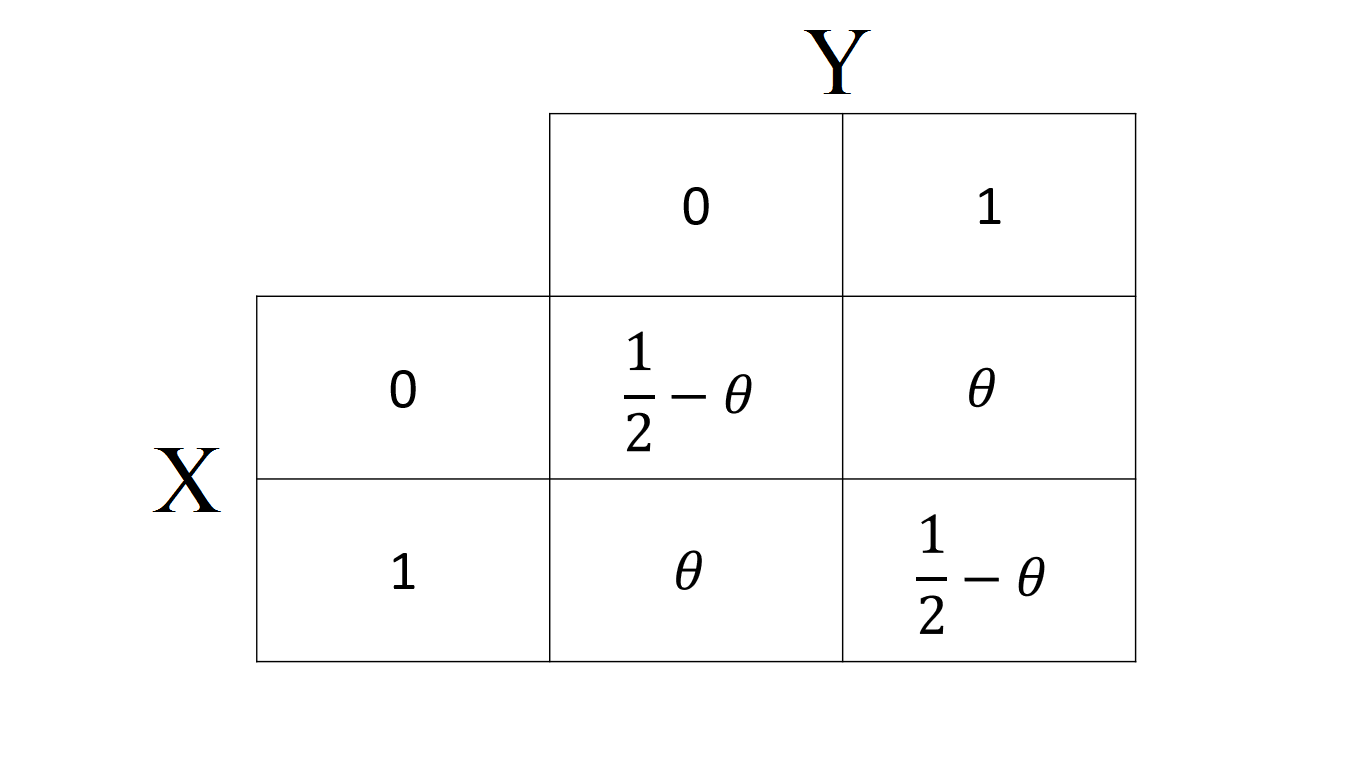
\includegraphics[width=100mm]{Q4_HW7}
%\end{center}
الف) توابع توزیع احتمال متغیرهای $X$ و $Y$ را به دست آورید.

ب) به ازای چه مقدار $\theta$ داریم
$$
P(X=Y)=1
$$
؟

پ) به ازای چه مقدار $\theta$ داریم
$$
P(X=x,Y=y)=P(X=x)P(Y=y)
$$
؟

سوال 1)

تعیین کنید به ازای چه مقادیری از $k$ هر یک از توابع زیر می تواند pdf یک متغیر تصادفی باشد.

الف) 
$
f(x)=\begin{cases}
1/x^k&,\quad x\ge 1\\
0&,\quad x<0
\end{cases}
$

ب)
$
f(x)=\begin{cases}
kxe^{-x}&,\quad x\ge 0\\
0&,\quad x<0
\end{cases}
$

پ)
$
f(x)=\begin{cases}
\sin x&,0\le x\le k\\
0&,\quad \text{سایر جاها}
\end{cases}
$
 ($k>0$)

ت)
$
f(x)=\begin{cases}
k\delta(x-1)&,\quad x=1\\
x&,\quad 0<x<1\\
0&,\quad \text{سایر جاها}
\end{cases}
$
(به عبارت دیگر، تابع در نقطه‌ی $x=1$ دارای ضربه‌ای به مساحت k است)

ث)
$
f(x)=k\delta(x-1)+(1-k)\delta(x)
$

سوال 2) یک سامانه دارای 70 قطعه است. پیشامد اینکه هر قطعه پس از شروع به کار در زمان 0، در بازه‌ی 
$
(0,x)
$
دچار خرابی گردد، یک متغیر تصادفی با pdf زیر است:
$$
f(x)=\begin{cases}
{1\over T}e^{-{x\over T}}&,\quad x\ge 0\\
0&,\quad x<0
\end{cases}
$$
احتمال آن را بیابید که بیش از 65 قطعه از این سیستم در بازه‌ی 
$
\left(0,{T\over 4}\right)
$
 دچار خرابی نشوند.

سوال 3) برای هر یک از pdf های سوال 1، مقدارهای 
$
\Pr\{X=1\}
$
و
$
\Pr\left\{X<{1\over 2}\right\}
$
را بیابید (پاسخ می تواند شامل ثابت k باشد).

سوال 4) اگر 
$
x_u
$
، صدک-u متغیر تصادفی 
$
X
$
باشد، در این صورت مقدار 
$
x_u
$
را به ازای 
$
u=0.2,0.4,0.6,0.8
$
برای حالت های زیر به دست آورید.

الف) 
$
X
$
یک متغیر تصادفی با pdf زیر است:
$$
f(x)=\begin{cases}
1&,\quad 0\le x\le 1\\
0&,\quad \text{سایر جاها}
\end{cases}
$$

ب) 
$
X
$
یک متغیر تصادفی با pdf زیر است:
$$
f(x)=\begin{cases}
2e^{-2x}&,\quad x\ge 0\\
0&,\quad \text{سایر جاها}
\end{cases}
$$

سوال 1) در پرتاب دو تاس سالم و متمایز، متغیر تصادفی $X$ را مجموع اعداد رو آمده و $Y$ را تعداد 6 های رو آمده در نظر بگیرید.

الف) مقدار 
$
\Pr\{X=1,Y=7\}
$
 را به دست آورید.

ب) مقدار 
$
E\{XY\}
$
 چقدر است؟

پ) (امتیازی) آیا این دو متغیر تصادفی ناهمبسته اند؟

سوال 2) در جدول زیر که توزیع احتمال را برای متغیر های تصادفی $X$ و $Y$ نشان می دهد،
\begin{table}[h]
\centering
\Large
\lr{
\begin{tabular}{|c|c|c|}
\hline
\backslashbox{$X$}{$Y$}&0&1\\\hline
0&$p_1$&$p_2$\\\hline
1&$p_3$&$p_4$\\\hline
\end{tabular}
}
\end{table}

الف) مقدار 
$
\text{\lr{cov}}(X,Y)
$
 را به دست آورید و تحقیق کنید کنید چه زمانی داریم 
$
\text{\lr{cov}}(X,Y)=0
$
؟

ب) آیا برای این دو متغیر تصادفی، ناهمبستگی، استقلال را نتیجه می دهد؟ اگر چنین است، نشان دهید و اگر چنین نیست، مثالی برای مقادیر 
$
p_1,p_2,p_3,p_4
$
 بزنید که ناهمبستگی، استقلال را نتیجه نمی‌دهد (دقت داشته باشید که جمع احتمالات برابر یک است و احتمالات نامنفی اند).

سوال 3) چگالی احتمال زیر را در نظر بگیرید:
$$
f_{X,Y}(x,y)=\begin{cases}
1+\alpha\sin[2\pi(x+y)]&,\quad 0\le x\le1,0\le y\le1
\\0&,\quad \text{در غیر این صورت}
\end{cases}
$$
که $\alpha$ مقدار مناسبی است.

الف) کوواریانس این دو متغیر تصادفی را به دست آورید. آیا این دو متغیر تصادفی ناهمبسته هستند؟

ب) مقادیری از $\alpha$ را بیابید که این دو متغیر تصادفی مستقل باشند.

سوال 4) تابع چگالی احتمال توام زیر را در نظر بگیرید:
$$
f_{X,Y}(x,y)={1\over 2\pi \sqrt{1-\rho^2}}\exp\left[-{1\over 2}\cdot{1\over 1-\rho^2}(x^2+y^2-2\rho xy)\right]
$$
الف) ثابت کنبد $X$ (و مشابها همچنین $Y$) دارای توزیع نرمال با میانگین صفر و واریانس $1$ است.

ب) ثابت کنید اگر $\rho=0$، در این صورت متغیرهای تصادفی $X$ و $Y$ مستقل هستند.

پ) (امتیازی) ثابت کنید اگر متغیرهای تصادفی $X$ و $Y$ مستقل باشند آنگاه $\rho=0$.

ت) (امتیازی تحقیقی) تابع چگالی احتمالی که در صورت این سوال تعریف شد، حالت خاصی از چگالی احتمال چند متغیره‌ی نرمال است.

ضریب همبستگی $\rho$ در حالت دو متغیره، میزان همبستگی دو متغیر تصادفی را نشان می دهد. ابتدا تحقیق کنید به ازای چه مقداری از $\rho$، این چگالی احتمال، دایروی-متقارن خواهد بود. چگالی احتمال دو متغیره را به ازای مقادیر 
$
\rho=-0.5,\rho=0,\rho=0.5
$
 ترسیم کنید. به طور شهودی چگونه می توان از روی نمودارها، به میزان همبستگی این دو متغیر تصادفی پی برد؟

این تابع چگالی را به صورت دیگری نیز می توان نوشت:
$$
f(x,y)={1\over \sqrt{(2\pi)^2}\det(\Sigma)}\exp\left[-{1\over 2}\cdot([x,y]\Sigma^{-1}[x,y]^T)\right]
$$
که بردار $[x,y]$ یک بردار سطری دوتایی است و 
$$
\Sigma=\begin{bmatrix}
1&\rho\\
\rho&1
\end{bmatrix}
$$
ماتریس $\Sigma$ در متغیرهای تصادفی نرمال توام، مفهوم مهمی است و ماتریس کوواریانس نام دارد.

به ازای هر یک از مقادیر 
$
\rho=-0.5,\rho=0,\rho=0.5
$
 و به کمک دستور 
\lr{mvnrnd()}
 در متلب، 1000 جفت داده‌ی تصادفی تولید و آنها را در یک نمودار پراکندگی ترسیم کنید (پس از اجرای دستور فوق در متلب به شیوه ی مناسب، 1000 داده‌ی تصادفی برای $X$ و 1000 داده‌ی تصادفی برای $Y$ خواهید داشت. کافی است $Y$ را برحسب $X$ رسم کنید تا به نمودار پراکندگی برسید. همچنین می توانید از \lr{Help} متلب برای توضیحات بیشتر در مورد \lr{mvnrnd()} بهره ببرید). چگونه از روی نمودار پراکندگی می توان میزان همبستگی دو متغیر تصادفی را نشان داد؟ چه شهودی در آن نهفته است؟

(این کار تحقیقی، امتیاز ویژه ای دارد و مهلت آن تا پایان امتحان نهایی خواهد بود؛ بنابراین زمان، محدودکننده نخواهد بود. بسیار مهم است که در این تحقیق، تحلیل و دیدگاه خود را نیز ذکر بفرمایید.)

هنگامی که $\rho=1$، توضیح دهید چه اتفاقی می افتد؟ تفاوت آن با حالت $\rho=-1$ چیست؟ آیا همچنان می‌توان از چگالی احتمال داده شده استفاده کرد؟ چرا؟

سوال 1) زمان خرابی یک لامپ، یک متغیر تصادفی با pdf زیر است:
$$
f_X(x)={1\over\lambda}e^{-{x\over\lambda}}\quad,\quad x>0
$$

الف) احتمال آن که این لامپ، به مدت حداکثر
$
2\lambda
$
عمر کند، چقدر است؟

ب) احتمال آن که این لامپ بیش از 
$
3\lambda
$
و کمتر از 
$
3.5\lambda
$
عمر کند چقدر است؟

سوال 2) یک متغیر تصادفی دارای چگالی احتمال زیر است:
$$
f_X(x)=\begin{cases}
6x^2(1-x)&,\quad 0\le x\le1\\
k\delta(x+1)&,\quad x=-1\\
0&,\quad \text{سایر جاها}
\end{cases}
$$
به عبارت دیگر، pdf دارای ضربه ای به اندازه k در $x=-1$ است.

الف) مقدار k را بیابید.

ب) CDF را به دست آورید و آن را رسم کنید.

پ) مقدار احتمال های 
$
\Pr\{-2< X\le {1\over2}\}
$
و
$
\Pr\{0< X\le {1\over2}\}
$
چقدر است؟

سوال 3) فرض کنید متغیر تصادفی $X$ دارای توزیع یکنواخت بین 0 و 1 است. در این صورت، CDF و pdf هر یک از متغیرهای تصادفی زیر را بیابید.

الف)
$
Y=X^2
$

ب)
$
Y=-\ln (1-X)
$

پ)
$
Y=\tan\pi (X-{1\over 2})
$

سوال 4) برای قسمت پ سوال پیش، مقدار احتمال های 
$
\Pr\{X\le {2\over 3}\}
$
و
$
\Pr\{Y\le {1\over \sqrt3}\}
$
را از روی pdf های X و Y بیابید و با هم مقایسه کنید. نتیجه مقایسه را توضیح دهید.
%(امتیازی: متغیرهای تصادفی بخش های ب و پ به کدام متغیرهای تصادفی معروف اشاره می کنند؟)

سوال 5) اگر CDF متغیر تصادفی X را با $F(x)$ نشان دهیم، CDF متغیرهای تصادفی زیر را برحسب $F(x)$ دست آورید.

الف)
$
Y=|X|
$
\quad\quad\quad\quad\quad
ب)
$
Y=\begin{cases}
0&,\quad X\le0\\
1&,\quad X>0
\end{cases}
$
\quad\quad\quad\quad\quad
پ)
$
Y=X^2-2X
$

%سوال 1) اگر متغیر های تصادفی $X$ و $Y$، دو جمله ای به ترتیب با پارامترهای 
%$
%(n_1,p)
%$
% و 
%$
%(n_2,p)
%$
% باشند،
%
%الف) با استفاده از تابع مولد گشتاور
%
%ب) بدون استفاده از تابع مولد گشتاور (به هر روش دلخواه)
%
%ثابت کنید متغیر تصادفی $X+Y$ دارای توزیع دوجمله ای با پارامترهای $
%(n_1+n_2,p)
%$
% است.
%\newline\newline
سوال 1) ابتدا فرض کنید متغیرهای تصادفی $X$ و $Y$ دارای توزیع یکنواخت در بازه‌ی $[0,1]$ و مستقل هستند. توزیع احتمال متغیرهای تصادفی 

الف) $XY$

ب) $X+Y$

پ) 
$
X\over Y
$

ت) 
$
\max\{X,Y\}
$

ج)
$
\min\{X,Y\}
$

را به دست آورید.

حال فرض کنید $X$ و $Y$ دو متغیر تصادفی نمایی و مستقل با پارامتر 1 باشند. توزیع احتمال هر یک از متغیرهای تصادفی قسمت ب) و پ) را بیابید.
%
%چ) $X+Y$
%
%ح) $X\over Y$
\newline\newline
سوال 2) توزیع مشترک دو متغیرتصادفی به صورت زیر است:
$$
f_{X,Y}(x,y)={1\over 2\pi \sqrt{1-\rho^2}}\exp\left[-{1\over 2}\cdot{1\over 1-\rho^2}(x^2+y^2-2\rho xy)\right]
$$
ثابت کنید متغیر تصادفی $X+Y$ یک متغیر تصادفی نرمال است و سپس واریانس آن را به دست آورید. چه زمانی این واریانس بیشینه است و چرا؟ در شرایطی که واریانس بیشینه باشد، متغیرهای تصادفی $X$ و $Y$ چه رابطه ای دارند؟
%\newline\newline
%سوال 4) برای دو متغیر تصادفی نمایی و مستقل $X$ و $Y$ با پارامتر 1، توزیع متغیرهای تصادفی زیر را به دست آورید:
%
%الف) $X+Y$
%
%ب) $X\over Y$

%پ) (امتیازی) $XY$

سوال 1) برای هر یک از متغیرهای تصادفی زیر، واریانس را به دست آورید.

الف) 
$
f_X(x)=\begin{cases}
e^{-x}&,\quad x>1\\
0&,\quad x\le1
\end{cases}
$

ب) 
$
f_X(x)=\begin{cases}
\sin x&,\quad 0<x<{\pi\over 2}\\
0&,\quad \text{سایر جاها}
\end{cases}
$

پ)
$
\begin{cases}
{2\over x^3}&,\quad x>1\\
0&,\quad \text{سایر جاها}
\end{cases}
$

ت) X یک متغیر تصادفی گسسته است و 
$
\Pr\{X=i\}=2({1\over 3})^i
$
برای 
$
i\in\Bbb N
$

سوال 2) برای قسمت های الف و ت سوال 1، ابتدا تابع مولد گشتاور را محاسبه نموده و سپس از روی آن، میانگین و واریانس را به دست آورید.

سوال 3) برای قسمت های الف و ب سوال 1، میانگین متغیر تصادفی $e^{-X}$ را بیابید.

سوال 4) برای هر یک از جفت متغیر های تصادفی $X$ و $Y$، ابتدا مقدار مناسب k و سپس مقدار 
$
\Pr\{X+3Y<{1\over 3}\}
$
را بیابید. در هر بخش آیا $X$ و $Y$ مستقلند؟ ($f_{X,Y}(x,y)$ چگالی احتمال توام متغیر های تصادفی پیوسته‌ی $X$ و $Y$ است.)

الف)
$
f_{X,Y}(x,y)=\begin{cases}
k\sin(x+3y)&,\quad 0<x<{\pi\over 2},0<y<{\pi\over 6}\\
0&,\quad \text{سایر جاها}
\end{cases}
$

ب)
$
f_{X,Y}(x,y)=\begin{cases}
kxy(1-y)&,\quad 0<x<1,0<y<1\\
0&,\quad \text{سایر جاها}
\end{cases}
$

سوال 5) جدول زیر را برای متغیرهای تصادفی $X$ و $Y$ در نظر بگیرید:
\begin{center}
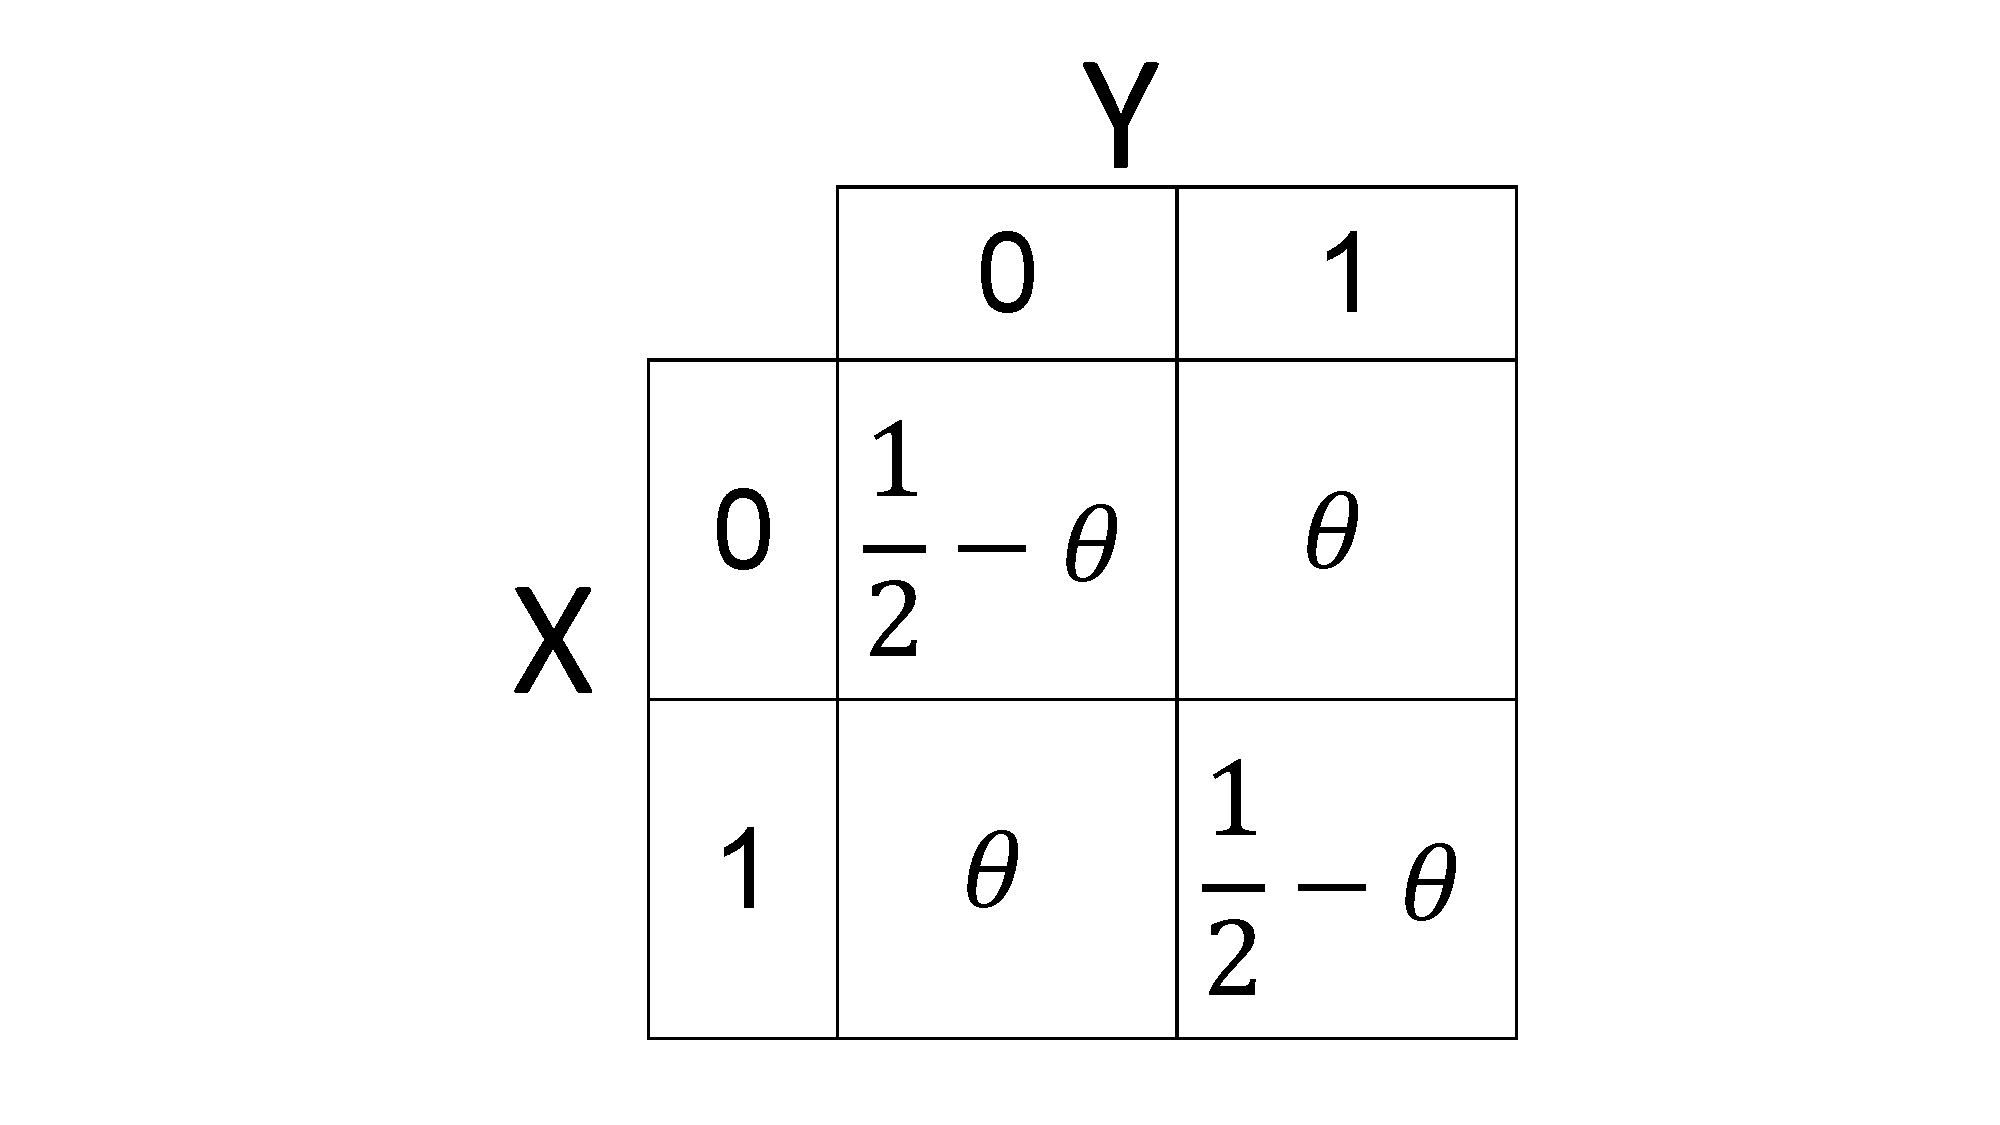
\includegraphics[width=70mm]{XY_CDF}
\end{center}
%\begin{latin}
%\begin{table}
%\centering
%{\huge
%\begin{tabular}{|c|c|c|}
%\hline
%&0&1\\
%\hline
%0&$\frac{1}{2}-\theta$&$\theta$\\
%\hline
%1&$\theta$&$\frac{1}{2}-\theta$\\
%\hline
%\end{tabular}
%}
%\end{table}
%\end{latin}
الف) توابع توزیع احتمال حاشیه ای متغیرهای $X$ و $Y$ را به دست آورید.

ب) به ازای چه مقدار $\theta$ داریم
$$
P(X=Y)=1
$$
؟

پ) به ازای چه مقدار $\theta$ داریم
$$
P(X=x,Y=y)=P(X=x)P(Y=y)
$$
؟

%سوال 1) اگر متغیر های تصادفی $X$ و $Y$، دو جمله ای به ترتیب با پارامترهای 
%$
%(n_1,p)
%$
% و 
%$
%(n_2,p)
%$
% باشند،
%
%الف) با استفاده از تابع مولد گشتاور
%
%ب) بدون استفاده از تابع مولد گشتاور (به هر روش دلخواه)
%
%ثابت کنید متغیر تصادفی $X+Y$ دارای توزیع دوجمله ای با پارامترهای $
%(n_1+n_2,p)
%$
% است.
%\newline\newline
سوال 1) در پرتاب 10 بار سکه‌ی سالم به طور مستقل،

الف) توزیع احتمال متغیر تصادفی تعداد سکه های شیر آمده را به شرط آن که بدانیم سه پرتاب اول خط بوده اند به دست آورید.

ب) توزیع احتمال متغیر تصادفی تعداد سکه های شیر آمده را به شرط آن که بدانیم دو پرتاب از سه پرتاب اول خط بوده اند به دست آورید.

سوال 2) کانال مخابراتی زیر را در نظر بگیرید:

\begin{figure}[h]
\centering
\Large
\lr{
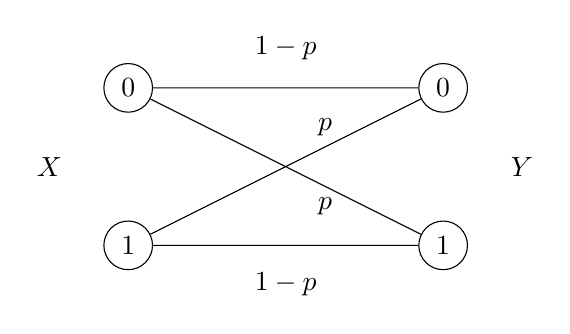
\begin{tikzpicture}
\node [draw=black,circle] (1) at(0,0) {0};
\node [draw=black,circle] (2) at(4,0) {0};
\node [draw=black,circle] (3) at(0,-2) {1};
\node [draw=black,circle] (4) at(4,-2) {1};
\draw 
(1) -- (2)
(1) -- (4)
(3) -- (2)
(3) -- (4)
;
\node (5) at(2,0.5) {$1-p$};
\node (6) at(2.5,-0.5) {$p$};
\node (7) at(2.5,-1.5) {$p$};
\node (8) at(2,-2.5) {$1-p$};
\node (9) at(-1,-1) {$X$};
\node (10) at(5,-1) {$Y$};
\end{tikzpicture}
}
\end{figure}
%\begin{center}
%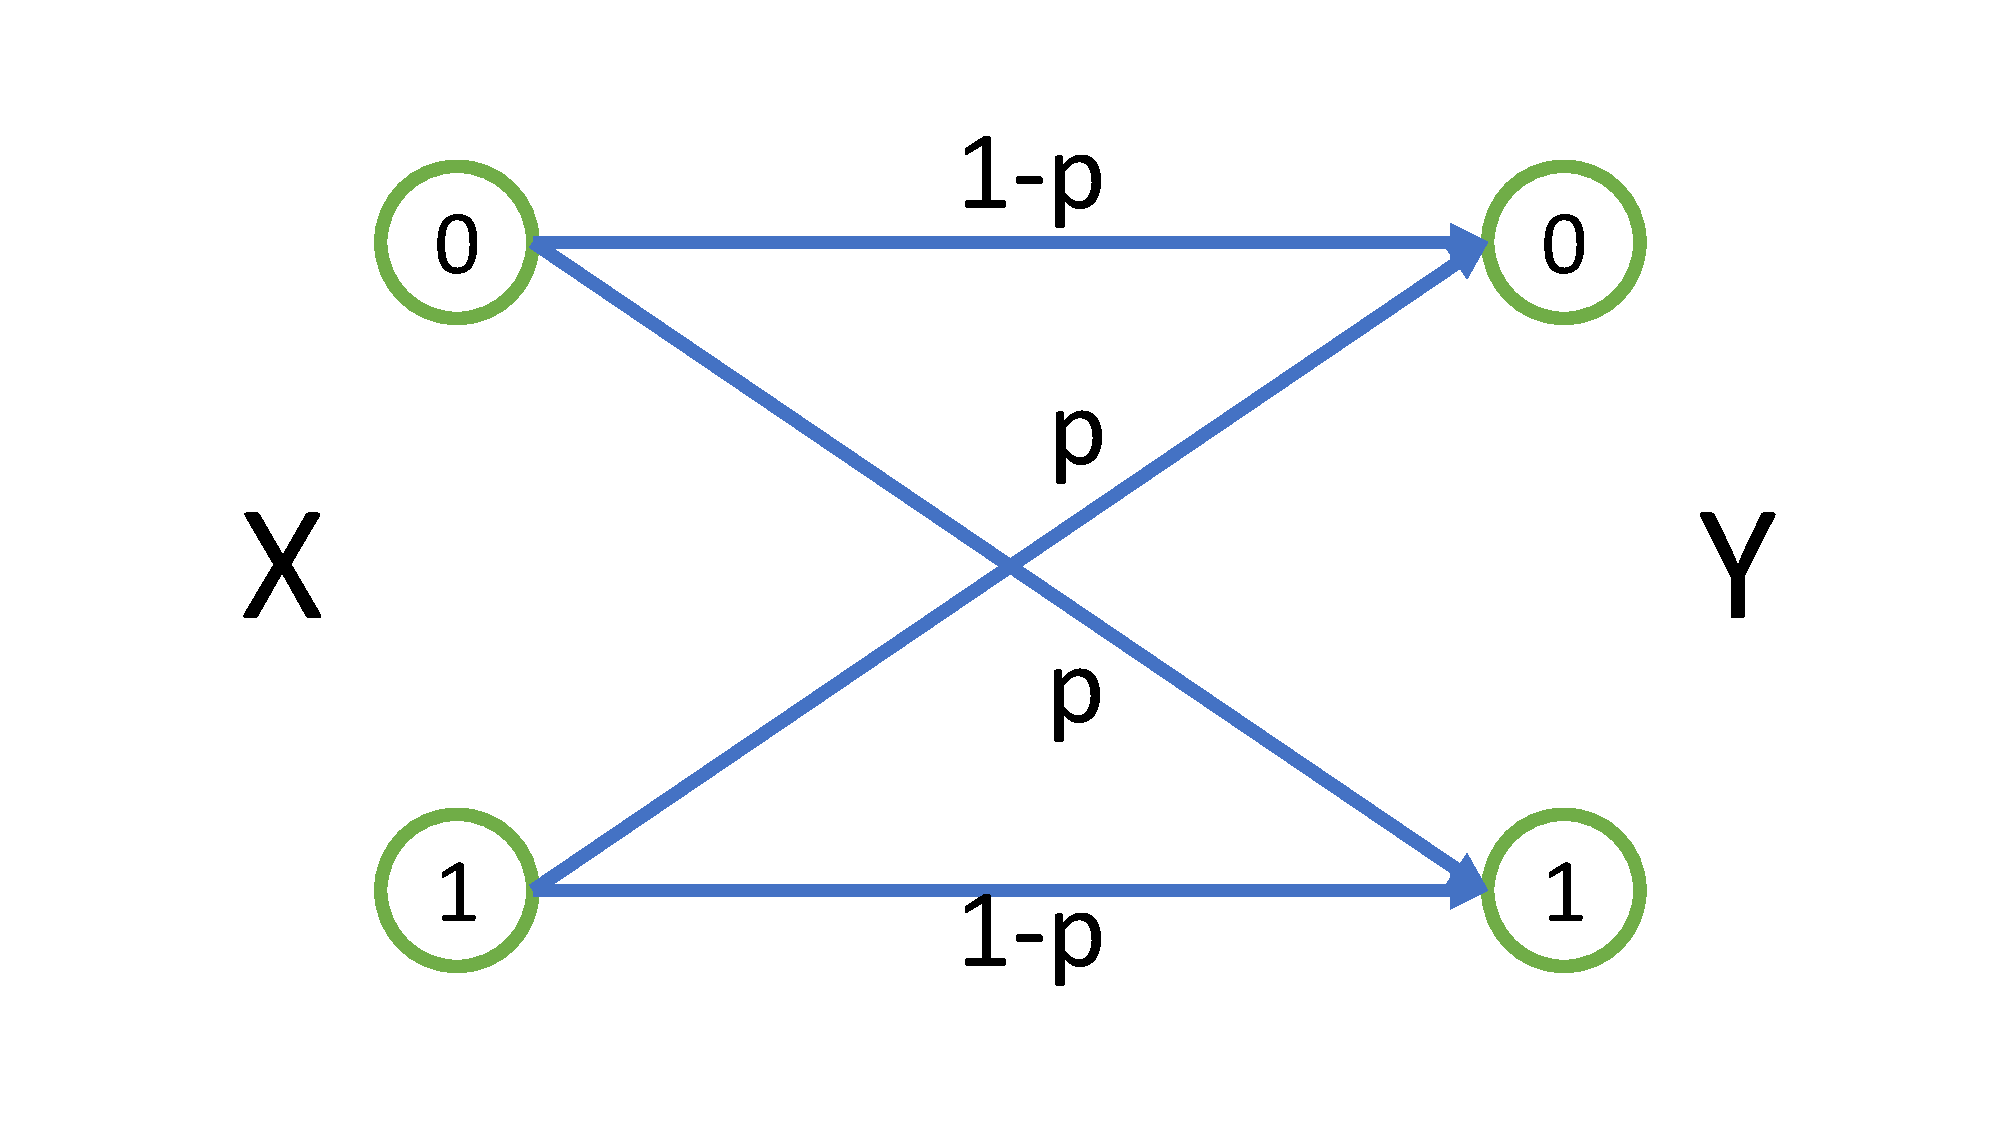
\includegraphics[width=80mm]{Q2_HW10.pdf}
%\end{center}
%\begin{tikzpicture}
%\centering
%\node[circle, draw=black, thick, inner sep=0pt, minimum size=30pt] (1) at (-1,1) {0};
%\node[circle, draw=black, thick, inner sep=0pt, minimum size=30pt] (2) at (1,1) {0};
%\node[circle, draw=black, thick, inner sep=0pt, minimum size=30pt] (3) at (-1,-1) {1};
%\node[circle, draw=black, thick, inner sep=0pt, minimum size=30pt] (4) at (1,-1) {1};
%\draw[->]
%(1)--node {$1-p$}(2)
%(1)--node {$p$}(4)
%(3)--node {$p$}(2)
%(3)--node {$1-p$}(4);
%\end{tikzpicture}
که در آن، پیکان ها احتمالات گذار را از متغیر تصادفی $X$ به متغیر تصادفی $Y$ نشان می دهند. به طور مثال
$$
\Pr\{Y=0|X=1\}=p
$$
الف) اگر 
$
\Pr\{X=0\}=q
$
 که 
$
0\le q\le 1
$
، در اینصورت توزیع توام $X$ و $Y$ را محاسبه کنید.

ب) احتمال خطا (
$
\Pr\{X\ne Y\}
$
)
 را محاسبه کنید. اگر مقدار $p$ ثابت باشد، آیا احتمال خطا بر حسب $q$ نقطه‌ی بهینه دارد؟ اگر دارد آنرا بیابید و در غیر این صورت، علت را بیان کنید.

سوال 3) فرض کنید متغیر تصادفی $X$ دارای توزیع احتمال نمایی با پارامتر $\lambda$ باشد. ثابت کنید
$$
E\{X|X>a\}=E\{X\}+a
$$

سوال 4) اگر توزیع تجمعی یک متغیر تصادفی ترکیبی به صورت 
$$
F(x)=\begin{cases}
0&,\quad x<0\\
{x+2\over 4}&,\quad 0\le x<1\\
1&,\quad x\ge 1
\end{cases}
$$
باشد، چگالی احتمال متغیر تصادفی 
$
X|(X\ne 0\text{\rl{ یا }}X\ne 1)
$
 را به دست آورید.

سوال 1) برای هر یک از pdf های توام داده شده‌ی زیر، موارد 
$
f_X(x)
$
،
$
E\{X\}
$
و
$
E\{XY\}
$
را به دست آورید.

الف) 
$
f_{X,Y}(x,y)=\frac{1}{\pi}e^{-x^2-y^2}
$

ب) 
$
f_{X,Y}(x,y)=\begin{cases}
\frac{3}{2}(1-|x-1|-|y-1|)&,\quad |x-1|+|y-1|<1\\
0&,\quad \text{سایر جاها}
\end{cases}
$

پ)
$
f_{X,Y}(x,y)=\begin{cases}
e^{1-x}&,\quad 0<x<y<1\\
0&,\quad \text{سایر جاها}
\end{cases}
$

ت) X و Y، دو متغیر تصادفی گسسته (با مقادیر صحیح) اند و pmf آنها به صورت زیر است:
$
p_{X,Y}(x,y)=\begin{cases}
\frac{1}{16}&,\quad x^2+y^2\le 10 \ \ ,\ \ x\ge y\\
0&,\quad \text{سایر جاها}
\end{cases}
$

سوال 2) در جدول زیر که توزیع احتمال را برای متغیر های تصادفی $X$ و $Y$ نشان می دهد،
\begin{center}
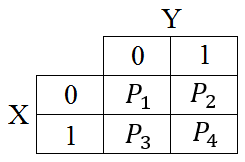
\includegraphics[width=40mm]{Q2_HW8}
\end{center}
الف) مقدار 
$
\text{\lr{cov}}(X,Y)
$
 را به دست آورید و تحقیق کنید کنید چه زمانی داریم 
$
\text{\lr{cov}}(X,Y)=0
$
؟

ب) آیا برای این دو متغیر تصادفی، ناهمبستگی، استقلال را نتیجه می دهد؟ اگر چنین است، نشان دهید و اگر چنین نیست، مثالی برای مقادیر 
$
p_1,p_2,p_3,p_4
$
 بزنید که ناهمبستگی، استقلال را نتیجه نمی‌دهد (دقت داشته باشید که جمع احتمالات برابر یک است و احتمالات نامنفی اند).
\newline
\newline
سوال 3) چگالی احتمال زیر را در نظر بگیرید:
$$
f_{X,Y}(x,y)=\begin{cases}
1+\alpha\sin[2\pi(x+y)]&,\quad 0\le x\le1,0\le y\le1
\\0&,\quad \text{در غیر این صورت}
\end{cases}
$$
که $\alpha$ مقدار مناسبی است.

الف) کوواریانس این دو متغیر تصادفی را به دست آورید. به ازای چه مقادیری از $\alpha$، این دو متغیر تصادفی ناهمبسته هستند؟

ب) مقادیری از $\alpha$ را بیابید که این دو متغیر تصادفی مستقل باشند.

سوال 4) ابتدا فرض کنید متغیرهای تصادفی $X$ و $Y$ دارای توزیع یکنواخت در بازه‌ی $[0,1]$ و مستقل هستند. توزیع احتمال متغیرهای تصادفی 

الف) $XY$

ب) $X+Y$

پ) (امتیازی)
$
X\over Y
$

ت) (امتیازی)
$
\max\{X,Y\}
$

ث) (امتیازی)
$
\min\{X,Y\}
$

را به دست آورید.

حال فرض کنید $X$ و $Y$ دو متغیر تصادفی نمایی و مستقل با پارامتر 1 باشند. توزیع احتمال هر یک از متغیرهای تصادفی قسمت ب و پ را بیابید (بخش پ همچنان امتیازی است!).

(توزیع احتمال یک متغیر تصادفی نمایی با پارامتر $\lambda$ به صورت زیر است:
$$
f(x)=\begin{cases}
\lambda e^{-\lambda x}&,\quad x>0\\
0&,\quad x\le0
\end{cases}
$$

توزیع احتمال یک متغیر تصادفی یکنواخت در بازه‌ی $[a,b]$ به صورت زیر است:
$$
f(x)=\begin{cases}
{1\over b-a}&,\quad a<x<b\\
0&,\quad \text{سایر جاها}
\end{cases}
$$
) 
%
%چ) $X+Y$
%
%ح) $X\over Y$

سوال 1) تابع چگالی احتمال توام دو متغیر تصادفی $X$ و $Y$ به صورت زیر است:
$$
f_{XY}(x,y)=\begin{cases}
k&,\quad |x|+|y|<1\\
0&,\quad \text{\rl{در غیر این صورت}}
\end{cases}
$$
الف) مقدار مناسب $k$ را بیابید.

ب) کوواریانس و ضریب همبستگی $X$ و $Y$ را بیابید.

پ) ثابت کنید متغیرهای تصادفی $X+Y$ و $X-Y$ مستقل هستند و توزیع توام آنها را به دست آورید.

ت) توزیع $X$ و میانگین و واریانس آن را به دست آورید.
\newline\newline
سوال 2) برای متغیر تصادفی $X$ که دارای توزیع زیر است
$$
f_X(x)=\begin{cases}
1&,\quad |x|<{1\over 2}\\
0&,\quad \text{\rl{در غیر این صورت}}
\end{cases}
$$
تابع مولد گشتاور را به دست آورده و از روی آن، $E\{X^4\}$ را محاسبه نمایید.
\newline\newline
سوال 3) ثابت کنید اگر $X,Y$، دو متغیر تصادفی نرمال مستقل با میانگین 0 و واریانس 1 باشند، آنگاه توزیع 
$
\tan^{-1}{Y\over X}
$
، یکنواخت بین $
-{\pi\over 2}
$
 و 
$
\pi\over 2
$
 خواهد بود.
\newline\newline
سوال 4) اگر برای متغیرهای تصادفی $X$ و $Y$، چگالی احتمال زیر را داشته باشیم
$$
f_{XY}(x,y)=\begin{cases}e^{-x(y+1)^2}&,\quad x,y>0\\
0&,\quad \text{\rl{در غیر این صورت}}\end{cases}
$$
در این صورت توزیع $X|Y$ را به دست آورید.
\newline\newline
سوال 5) (امتیازی) تحقیق کنید هر یک از دنباله‌ی متغیرهای تصادفی زیر، با چه مفهومی به یک متغیر تصادفی حدی میل می کنند. برای هر یک دلیل بیاورید.

الف) 
$
X_n=X+{1\over n}
$
 که $X$، یک متغیر تصادفی یکنواخت در بازه‌ی $[0,1]$ است.

ب) متغیر تصادفی نمایی با پارامتر ${n+1\over n}$

پ) متوسط تعداد شیرها در $n$ بار پرتاب مستقل یک سکه‌ی سالم

سوال 1) اگر متغیر تصادفی 
$
X
$
را دارای چگالی احتمال زیر در نظر بگیریم
\eqn{
f_X(x)=\begin{cases}
{1\over 2}&,\quad 0<x<2\\
0&,\quad \text{سایر جاها}
\end{cases}
}
موارد 
$
F(x|X<1)
$
(cdf)
،
$
f(x|X>1)
$
(pdf)
و
$
\mathbb{E}\{X|0.5<X<1.5\}
$
را بیابید.

سوال 2) فرض کنید متغیر تصادفی 
$
X
$
 دارای چگالی احتمال زیر باشد
\eqn{
f_X(x)=
\begin{cases}
\lambda e^{-\lambda x} &,\quad x>0\\
0&,\quad \text{سایر جاها}
\end{cases} \quad,\quad \lambda>0
}
در این صورت مقادیر 
$
\mathbb{E}\{X|X>a\}
$
و
$
\mathbb{E}\{X\}+a
$
را بیابید و با هم مقایسه کنید.

(امتیازی: نتیجه را تفسیر کنید و ببینید آیا با شهود سازگار است. این چه ویژگی ای از متغیرهای تصادفی نمایی را نشان می دهد؟)

سوال 3) برای متغیر تصادفی 
$
X
$
با توزیع زیر
\eqn{
\Pr\{X=i\}=(1-p)^i\cdot p\quad,\quad i=0,1,2,\cdots
}
الف) مقدار 
$
\text{var}\{X|X\ge 4\}
$
را به دست آورید.

ب) pmf شرطی 
$
\Pr\{X=x|\text{X زوج است}\}
$
را پیدا کنید.

سوال 4) فرض کنید متغیر تصادفی $X$، نتیجه پرتاب یک تاس سالم باشد (
$
X\in\{1,2,3,4,5,6\}
$
).
سپس با توجه به رخداد 
$
X
$
، متغیر تصادفی پیوسته‌ی
$
Y
$
را به صورت شرطی با چگالی احتمال زیر تعریف می کنیم:
\eqn{
f_{Y|X}(x,y)=\begin{cases}
{1\over x}&,\quad 0<y<x\\
0&,\quad \text{سایر جاها}
\end{cases}
}

الف) احتمال 
$
\Pr\{Y\ge 3\}
$
را بیابید.

ب) چگالی احتمال 
$
f_Y(y)
$
را به دست آورید.

پ) مقادیر 
$
\mathbb{E}\{Y\}
$
و
$
\text{var}(Y)
$
را از روی چگالی احتمال $Y$ محاسبه کنید.

\Q

از کیسه‌ای که شامل 5 مهره سیاه، 8 مهره سفید و 1 مهره قرمز است، دو توپ به تصادف بیرون می‌آوریم. احتمال آنکه هر دو توپ همرنگ باشند چقدر است؟

\Q

دو جعبه از لامپ‌ها در اختیار داریم. جعبه‌ی اول، دارای 1000 لامپ است که $1\%$ آنها سالمند. جعبه‌ی دوم، دارای 10000 لامپ است که $95\%$ آنها سالم اند. یکی از جعبه‌ها را به تصادف انتخاب کرده و دو لامپ بیرون می‌کشیم. احتمال آن که هر دو لامپ از جعبه‌ی 1 انتخاب شده باشند چقدر است اگر

الف) هر دو لامپ خراب باشند.

ب) اگر یکی از لامپ ها سالم و دیگری خراب باشد.



\Q

سکه‌ای را پرتاب می‌کنیم. اگر رو آمد، آن را 9 بار دیگر پرتاب می‌کنیم و نتایج 10 پرتاب را در نظر می‌گیریم. اگر پشت آمد، آن را 5 بار دیگر پرتاب می‌کنیم و نتایج 6 پرتاب را در نظر می‌گیریم. احتمال آن که در تمام پرتاب های سکه، دقیقا 6 بار رو بیاید چقدر است؟

\Q

یک آزمایش برنولی را که احتمال موفقیت در آن برابر 
$
40\%
$
است، $n$ بار تکرار می‌کنیم. اگر $k$، برابر تعداد موفقیت‌ها در این پرتاب ها باشد، $n$ حداقل چقدر باشد تا احتمال رخداد 
$
\{38\%<\frac{k}{n}<42\%\}
$
بیش از 
$
70\%
$
باشد؟

(راهنمایی: از قضیه‌ی دموآور-لاپلاس استفاده نمایید.)

(جدول مربوط به محاسبه‌ی تابع 
$
G^{-1}(x)
$
در صفحه‌ی بعد آمده است.
)

\newpage

\newgeometry{left=0mm,right=0mm}

%\begin{figure}[h]
%\centering
%\includegraphics[width=220mm]{ginv.pdf}
%\end{figure}

%(تنها نامساوی مربوط به قضیه‌ی دموآور-لاپلاس را نوشته، اعداد را جایگذاری نموده و ساده کنید. محاسبه‌ی دقیق مقدار $n$ الزامی نیست.)
%سکه‌ای را پرتاب می‌کنیم. اگر رو آمد، یک تاس سالم را 5 بار پرتاب کرده و جمع اعداد این 5 پرتاب را می‌نویسیم.

\begin{table}[h]
\centering
\large
\lr{
\begin{tabular}{|c|c|c|c|c|c|c|c|}
\hline
$x$&$G^{-1}(x)$&$x$&$G^{-1}(x)$&$x$&$G^{-1}(x)$&$x$&$G^{-1}(x)$\\\hline
0.01&-2.3263&0.26&-0.6433&0.51&0.0251&0.76&0.7063\\\hline
0.02&-2.0537&0.27&-0.6128&0.52&0.0502&0.77&0.7388\\\hline
0.03&-1.8808&0.28&-0.5828&0.53&0.0753&0.78&0.7722\\\hline
0.04&-1.7507&0.29&-0.5534&0.54&0.1004&0.79&0.8064\\\hline
0.05&-1.6449&0.30&-0.5244&0.55&0.1257&0.80&0.8416\\\hline
0.06&-1.5548&0.31&-0.4959&0.56&0.1510&0.81&0.8779\\\hline
0.07&-1.4758&0.32&-0.4677&0.57&0.1764&0.82&0.9154\\\hline
0.08&-1.4051&0.33&-0.4399&0.58&0.2019&0.83&0.9542\\\hline
0.09&-1.3408&0.34&-0.4125&0.59&0.2275&0.84&0.9945\\\hline
0.10&-1.2816&0.35&-0.3853&0.60&0.2533&0.85&1.0364\\\hline
0.11&-1.2265&0.36&-0.3585&0.61&0.2793&0.86&1.0803\\\hline
0.12&-1.1750&0.37&-0.3319&0.62&0.3055&0.87&1.1264\\\hline
0.13&-1.1264&0.38&-0.3055&0.63&0.3319&0.88&1.1750\\\hline
0.14&-1.0803&0.39&-0.2793&0.64&0.3585&0.89&1.2265\\\hline
0.15&-1.0364&0.40&-0.2533&0.65&0.3853&0.90&1.2816\\\hline
0.16&-0.9945&0.41&-0.2275&0.66&0.4125&0.91&1.3408\\\hline
0.17&-0.9542&0.42&-0.2019&0.67&0.4399&0.92&1.4051\\\hline
0.18&-0.9154&0.43&-0.1764&0.68&0.4677&0.93&1.4758\\\hline
0.19&-0.8779&0.44&-0.1510&0.69&0.4959&0.94&1.5548\\\hline
0.20&-0.8416&0.45&-0.1257&0.70&0.5244&0.95&1.6449\\\hline
0.21&-0.8064&0.46&-0.1004&0.71&0.5534&0.96&1.7507\\\hline
0.22&-0.7722&0.47&-0.0753&0.72&0.5828&0.97&1.8808\\\hline
0.23&-0.7388&0.48&-0.0502&0.73&0.6128&0.98&2.0537\\\hline
0.24&-0.7063&0.49&-0.0251&0.74&0.6433&0.99&2.3263\\\hline
0.25&-0.6745&0.50&0.0000&0.75&0.6745&0.9999&3.7190\\\hline
\end{tabular}
}
\end{table}


\end{document}